\documentclass[12pt]{article}

% House style preamble
% !TEX TS-program = xelatex
% File: preamble.tex
% Purpose: Brett Reynolds house style LaTeX preamble
% Version: 2.0.0 (December 2025 typography redesign)
%
% Usage: % !TEX TS-program = xelatex
% File: preamble.tex
% Purpose: Brett Reynolds house style LaTeX preamble
% Version: 2.0.0 (December 2025 typography redesign)
%
% Usage: % !TEX TS-program = xelatex
% File: preamble.tex
% Purpose: Brett Reynolds house style LaTeX preamble
% Version: 2.0.0 (December 2025 typography redesign)
%
% Usage: \input{.house-style/preamble.tex} in main document
%
% Compiler: XeLaTeX (default) or LuaLaTeX
%           NOT pdfLaTeX - requires fontspec for fonts

% ===========================
% FONTS
% ===========================
\usepackage{fontspec}

\setmainfont{EB Garamond}[
  Numbers=OldStyle,
  Ligatures=TeX,
  BoldFont={EB Garamond},
]

% IPA fallback font
\newfontfamily\ipafont{Charis SIL}
\newcommand{\ipa}[1]{{\ipafont #1}}

% CJK fallback font (Japanese / Chinese / Korean)
% BUILD VALIDATION ONLY: unused CJK fallback replaced because Hiragino is unavailable.
\newfontfamily\cjkfont{DejaVu Sans}
\newcommand{\cjk}[1]{{\cjkfont #1}}

% Lining figures when needed (tables, years in isolation)
\providecommand{\liningnums}[1]{{\addfontfeatures{Numbers=Lining}#1}}

% Monospace
\setmonofont{Inconsolata}[Scale=MatchLowercase]

% ===========================
% PAGE LAYOUT
% ===========================
\usepackage[
  letterpaper,
  inner=1.25in,
  outer=1in,
  top=1in,
  bottom=1.25in,
  marginparwidth=0.6in,
]{geometry}

\usepackage[british]{babel} % Oxford spelling: -ize where standard, British punctuation/hyphenation
\usepackage[final]{microtype}

% ===========================
% HEADINGS
% ===========================
\usepackage{titlesec}

% Section: small caps, number in margin
\titleformat{\section}
  {\normalfont\scshape}
  {\llap{\thesection\quad}}
  {0pt}
  {}

% Subsection: small caps sentence case
\titleformat{\subsection}
  {\normalfont\normalsize\scshape}
  {\thesubsection\quad}
  {0pt}
  {}

% Subsubsection: upright
\titleformat{\subsubsection}
  {\normalfont}
  {\thesubsubsection\quad}
  {0pt}
  {}

% Spacing
\titlespacing*{\section}{0pt}{2ex plus 1ex minus .2ex}{1ex plus .2ex}
\titlespacing*{\subsection}{0pt}{1.5ex plus 1ex minus .2ex}{0.5ex plus .2ex}
\titlespacing*{\subsubsection}{0pt}{1ex plus 0.5ex minus .1ex}{0.3ex plus .1ex}

% ===========================
% RUNNING HEADS
% ===========================
\usepackage{fancyhdr}
\pagestyle{fancy}
\fancyhf{}
\renewcommand{\sectionmark}[1]{%
  \markboth{\ifnum\value{secnumdepth}>0 \thesection\quad\fi #1}{}%
}
\fancyhead[LE]{\small\scshape\leftmark}
\fancyhead[RO]{\small\scshape\@title}
\fancyfoot[LE,RO]{\thepage}
\renewcommand{\headrulewidth}{0pt}

% For oneside documents (most papers):
\fancyhead[L]{\small\scshape\leftmark}
\fancyhead[R]{\small\thepage}
\fancyfoot{}

% ===========================
% COLORS & HYPERLINKS
% ===========================
\usepackage{xcolor}
\definecolor{linkmaroon}{RGB}{128, 0, 32}

\usepackage{hyperref}
% BUILD VALIDATION: permit line breaks in long repository file paths.
\usepackage{xurl}
\hypersetup{
  colorlinks=true,
  linkcolor=linkmaroon,
  citecolor=linkmaroon,
  urlcolor=linkmaroon,
  pdfauthor={Brett Reynolds},
}

\usepackage{orcidlink}

% ===========================
% QUOTATIONS
% ===========================
\usepackage[style=american]{csquotes} % Double quotes outer (Oxford spelling kept via babel)
\MakeOuterQuote{"}

% ===========================
% SEMANTIC MACROS
% ===========================
% Terms (linguistic concepts being introduced/defined)
\newcommand{\term}[1]{\textsc{#1}}

% Mentions (words/expressions under discussion)
\newcommand{\mention}[1]{\textit{#1}}

% Mentions in headings (robust italic form)
% Robust: headings are moving arguments (written to .toc/.aux)
\DeclareRobustCommand{\mentionhead}[1]{\texorpdfstring{{\normalfont\itshape\NoCaseChange{#1}}}{#1}}

% Object language (cited forms, foreign words)
\newcommand{\olang}[1]{\textit{#1}}

% Small-caps abbreviations for glosses
\newcommand{\abbr}[1]{\textsc{#1}}

% Cross-linguistic subscript marker
\usepackage{marvosym}
\newcommand{\crossmark}{\textsubscript{\Cross}}

% ===========================
% MATHS AND SYMBOLS
% ===========================
\usepackage{amsmath,amssymb}

% ===========================
% LINGUISTIC EXAMPLES
% ===========================
\usepackage{langsci-gb4e}
\makeatletter
\@ifundefined{noautomath}{}{\noautomath}
\makeatother

% Judgement markers
\newcommand{\ungram}[1]{*\!#1}
\newcommand{\marg}[1]{?\!#1}
\newcommand{\odd}[1]{\#\!#1}

% ===========================
% LISTS
% ===========================
\usepackage{enumitem}
\setlist{nosep, leftmargin=*}
\setlist[enumerate]{label=\arabic*.}
\setlist[itemize]{label=--}

% ===========================
% TABLES & FIGURES
% ===========================
\usepackage{booktabs}
\usepackage{array}
\usepackage{graphicx}
\graphicspath{{figures/}}

% ===========================
% BIBLIOGRAPHY
% ===========================
\usepackage[backend=biber,style=apa,natbib=true,doi=true,isbn=false,url=true]{biblatex}
\IfFileExists{references-standalone.bib}
  {\addbibresource{references-standalone.bib}}
  {\addbibresource{references.bib}\IfFileExists{references-local.bib}{\addbibresource{references-local.bib}}{}}

% Possessive citation: Author's (Year)
\newcommand{\posscite}[1]{\citeauthor{#1}'s (\citeyear{#1})}

% ===========================
% UTILITIES
% ===========================
\usepackage{xspace}
\newcommand{\eg}{e.g.,\xspace}
\newcommand{\ie}{i.e.,\xspace}
\newcommand{\etc}{etc.\xspace}

% ===========================
% AI-USE DISCLOSURE
% ===========================
% House style: place on page 1, immediately after the abstract/keywords, so the
% AI involvement is visible to the reader up front rather than buried at the end.
% Argument is the model list (use CURRENT names; frontier names change fast).
%   \aidisclosure{Claude 4.5 \& Opus 4.8; ChatGPT 5.2 pro; Gemini 3; DeepSeek V3}
\newcommand{\aidisclosure}[1]{%
  \par\medskip
  \noindent{\small\textsc{AI use.}\enspace The large language models #1 served as
  drafting and editing aids throughout the preparation of this paper. I am
  responsible for all theoretical claims, arguments, errors, and interpretive
  choices.\par}%
  \medskip
}

 in main document
%
% Compiler: XeLaTeX (default) or LuaLaTeX
%           NOT pdfLaTeX - requires fontspec for fonts

% ===========================
% FONTS
% ===========================
\usepackage{fontspec}

\setmainfont{EB Garamond}[
  Numbers=OldStyle,
  Ligatures=TeX,
  BoldFont={EB Garamond},
]

% IPA fallback font
\newfontfamily\ipafont{Charis SIL}
\newcommand{\ipa}[1]{{\ipafont #1}}

% CJK fallback font (Japanese / Chinese / Korean)
% BUILD VALIDATION ONLY: unused CJK fallback replaced because Hiragino is unavailable.
\newfontfamily\cjkfont{DejaVu Sans}
\newcommand{\cjk}[1]{{\cjkfont #1}}

% Lining figures when needed (tables, years in isolation)
\providecommand{\liningnums}[1]{{\addfontfeatures{Numbers=Lining}#1}}

% Monospace
\setmonofont{Inconsolata}[Scale=MatchLowercase]

% ===========================
% PAGE LAYOUT
% ===========================
\usepackage[
  letterpaper,
  inner=1.25in,
  outer=1in,
  top=1in,
  bottom=1.25in,
  marginparwidth=0.6in,
]{geometry}

\usepackage[british]{babel} % Oxford spelling: -ize where standard, British punctuation/hyphenation
\usepackage[final]{microtype}

% ===========================
% HEADINGS
% ===========================
\usepackage{titlesec}

% Section: small caps, number in margin
\titleformat{\section}
  {\normalfont\scshape}
  {\llap{\thesection\quad}}
  {0pt}
  {}

% Subsection: small caps sentence case
\titleformat{\subsection}
  {\normalfont\normalsize\scshape}
  {\thesubsection\quad}
  {0pt}
  {}

% Subsubsection: upright
\titleformat{\subsubsection}
  {\normalfont}
  {\thesubsubsection\quad}
  {0pt}
  {}

% Spacing
\titlespacing*{\section}{0pt}{2ex plus 1ex minus .2ex}{1ex plus .2ex}
\titlespacing*{\subsection}{0pt}{1.5ex plus 1ex minus .2ex}{0.5ex plus .2ex}
\titlespacing*{\subsubsection}{0pt}{1ex plus 0.5ex minus .1ex}{0.3ex plus .1ex}

% ===========================
% RUNNING HEADS
% ===========================
\usepackage{fancyhdr}
\pagestyle{fancy}
\fancyhf{}
\renewcommand{\sectionmark}[1]{%
  \markboth{\ifnum\value{secnumdepth}>0 \thesection\quad\fi #1}{}%
}
\fancyhead[LE]{\small\scshape\leftmark}
\fancyhead[RO]{\small\scshape\@title}
\fancyfoot[LE,RO]{\thepage}
\renewcommand{\headrulewidth}{0pt}

% For oneside documents (most papers):
\fancyhead[L]{\small\scshape\leftmark}
\fancyhead[R]{\small\thepage}
\fancyfoot{}

% ===========================
% COLORS & HYPERLINKS
% ===========================
\usepackage{xcolor}
\definecolor{linkmaroon}{RGB}{128, 0, 32}

\usepackage{hyperref}
% BUILD VALIDATION: permit line breaks in long repository file paths.
\usepackage{xurl}
\hypersetup{
  colorlinks=true,
  linkcolor=linkmaroon,
  citecolor=linkmaroon,
  urlcolor=linkmaroon,
  pdfauthor={Brett Reynolds},
}

\usepackage{orcidlink}

% ===========================
% QUOTATIONS
% ===========================
\usepackage[style=american]{csquotes} % Double quotes outer (Oxford spelling kept via babel)
\MakeOuterQuote{"}

% ===========================
% SEMANTIC MACROS
% ===========================
% Terms (linguistic concepts being introduced/defined)
\newcommand{\term}[1]{\textsc{#1}}

% Mentions (words/expressions under discussion)
\newcommand{\mention}[1]{\textit{#1}}

% Mentions in headings (robust italic form)
% Robust: headings are moving arguments (written to .toc/.aux)
\DeclareRobustCommand{\mentionhead}[1]{\texorpdfstring{{\normalfont\itshape\NoCaseChange{#1}}}{#1}}

% Object language (cited forms, foreign words)
\newcommand{\olang}[1]{\textit{#1}}

% Small-caps abbreviations for glosses
\newcommand{\abbr}[1]{\textsc{#1}}

% Cross-linguistic subscript marker
\usepackage{marvosym}
\newcommand{\crossmark}{\textsubscript{\Cross}}

% ===========================
% MATHS AND SYMBOLS
% ===========================
\usepackage{amsmath,amssymb}

% ===========================
% LINGUISTIC EXAMPLES
% ===========================
\usepackage{langsci-gb4e}
\makeatletter
\@ifundefined{noautomath}{}{\noautomath}
\makeatother

% Judgement markers
\newcommand{\ungram}[1]{*\!#1}
\newcommand{\marg}[1]{?\!#1}
\newcommand{\odd}[1]{\#\!#1}

% ===========================
% LISTS
% ===========================
\usepackage{enumitem}
\setlist{nosep, leftmargin=*}
\setlist[enumerate]{label=\arabic*.}
\setlist[itemize]{label=--}

% ===========================
% TABLES & FIGURES
% ===========================
\usepackage{booktabs}
\usepackage{array}
\usepackage{graphicx}
\graphicspath{{figures/}}

% ===========================
% BIBLIOGRAPHY
% ===========================
\usepackage[backend=biber,style=apa,natbib=true,doi=true,isbn=false,url=true]{biblatex}
\IfFileExists{references-standalone.bib}
  {\addbibresource{references-standalone.bib}}
  {\addbibresource{references.bib}\IfFileExists{references-local.bib}{\addbibresource{references-local.bib}}{}}

% Possessive citation: Author's (Year)
\newcommand{\posscite}[1]{\citeauthor{#1}'s (\citeyear{#1})}

% ===========================
% UTILITIES
% ===========================
\usepackage{xspace}
\newcommand{\eg}{e.g.,\xspace}
\newcommand{\ie}{i.e.,\xspace}
\newcommand{\etc}{etc.\xspace}

% ===========================
% AI-USE DISCLOSURE
% ===========================
% House style: place on page 1, immediately after the abstract/keywords, so the
% AI involvement is visible to the reader up front rather than buried at the end.
% Argument is the model list (use CURRENT names; frontier names change fast).
%   \aidisclosure{Claude 4.5 \& Opus 4.8; ChatGPT 5.2 pro; Gemini 3; DeepSeek V3}
\newcommand{\aidisclosure}[1]{%
  \par\medskip
  \noindent{\small\textsc{AI use.}\enspace The large language models #1 served as
  drafting and editing aids throughout the preparation of this paper. I am
  responsible for all theoretical claims, arguments, errors, and interpretive
  choices.\par}%
  \medskip
}

 in main document
%
% Compiler: XeLaTeX (default) or LuaLaTeX
%           NOT pdfLaTeX - requires fontspec for fonts

% ===========================
% FONTS
% ===========================
\usepackage{fontspec}

\setmainfont{EB Garamond}[
  Numbers=OldStyle,
  Ligatures=TeX,
  BoldFont={EB Garamond},
]

% IPA fallback font
\newfontfamily\ipafont{Charis SIL}
\newcommand{\ipa}[1]{{\ipafont #1}}

% CJK fallback font (Japanese / Chinese / Korean)
% BUILD VALIDATION ONLY: unused CJK fallback replaced because Hiragino is unavailable.
\newfontfamily\cjkfont{DejaVu Sans}
\newcommand{\cjk}[1]{{\cjkfont #1}}

% Lining figures when needed (tables, years in isolation)
\providecommand{\liningnums}[1]{{\addfontfeatures{Numbers=Lining}#1}}

% Monospace
\setmonofont{Inconsolata}[Scale=MatchLowercase]

% ===========================
% PAGE LAYOUT
% ===========================
\usepackage[
  letterpaper,
  inner=1.25in,
  outer=1in,
  top=1in,
  bottom=1.25in,
  marginparwidth=0.6in,
]{geometry}

\usepackage[british]{babel} % Oxford spelling: -ize where standard, British punctuation/hyphenation
\usepackage[final]{microtype}

% ===========================
% HEADINGS
% ===========================
\usepackage{titlesec}

% Section: small caps, number in margin
\titleformat{\section}
  {\normalfont\scshape}
  {\llap{\thesection\quad}}
  {0pt}
  {}

% Subsection: small caps sentence case
\titleformat{\subsection}
  {\normalfont\normalsize\scshape}
  {\thesubsection\quad}
  {0pt}
  {}

% Subsubsection: upright
\titleformat{\subsubsection}
  {\normalfont}
  {\thesubsubsection\quad}
  {0pt}
  {}

% Spacing
\titlespacing*{\section}{0pt}{2ex plus 1ex minus .2ex}{1ex plus .2ex}
\titlespacing*{\subsection}{0pt}{1.5ex plus 1ex minus .2ex}{0.5ex plus .2ex}
\titlespacing*{\subsubsection}{0pt}{1ex plus 0.5ex minus .1ex}{0.3ex plus .1ex}

% ===========================
% RUNNING HEADS
% ===========================
\usepackage{fancyhdr}
\pagestyle{fancy}
\fancyhf{}
\renewcommand{\sectionmark}[1]{%
  \markboth{\ifnum\value{secnumdepth}>0 \thesection\quad\fi #1}{}%
}
\fancyhead[LE]{\small\scshape\leftmark}
\fancyhead[RO]{\small\scshape\@title}
\fancyfoot[LE,RO]{\thepage}
\renewcommand{\headrulewidth}{0pt}

% For oneside documents (most papers):
\fancyhead[L]{\small\scshape\leftmark}
\fancyhead[R]{\small\thepage}
\fancyfoot{}

% ===========================
% COLORS & HYPERLINKS
% ===========================
\usepackage{xcolor}
\definecolor{linkmaroon}{RGB}{128, 0, 32}

\usepackage{hyperref}
% BUILD VALIDATION: permit line breaks in long repository file paths.
\usepackage{xurl}
\hypersetup{
  colorlinks=true,
  linkcolor=linkmaroon,
  citecolor=linkmaroon,
  urlcolor=linkmaroon,
  pdfauthor={Brett Reynolds},
}

\usepackage{orcidlink}

% ===========================
% QUOTATIONS
% ===========================
\usepackage[style=american]{csquotes} % Double quotes outer (Oxford spelling kept via babel)
\MakeOuterQuote{"}

% ===========================
% SEMANTIC MACROS
% ===========================
% Terms (linguistic concepts being introduced/defined)
\newcommand{\term}[1]{\textsc{#1}}

% Mentions (words/expressions under discussion)
\newcommand{\mention}[1]{\textit{#1}}

% Mentions in headings (robust italic form)
% Robust: headings are moving arguments (written to .toc/.aux)
\DeclareRobustCommand{\mentionhead}[1]{\texorpdfstring{{\normalfont\itshape\NoCaseChange{#1}}}{#1}}

% Object language (cited forms, foreign words)
\newcommand{\olang}[1]{\textit{#1}}

% Small-caps abbreviations for glosses
\newcommand{\abbr}[1]{\textsc{#1}}

% Cross-linguistic subscript marker
\usepackage{marvosym}
\newcommand{\crossmark}{\textsubscript{\Cross}}

% ===========================
% MATHS AND SYMBOLS
% ===========================
\usepackage{amsmath,amssymb}

% ===========================
% LINGUISTIC EXAMPLES
% ===========================
\usepackage{langsci-gb4e}
\makeatletter
\@ifundefined{noautomath}{}{\noautomath}
\makeatother

% Judgement markers
\newcommand{\ungram}[1]{*\!#1}
\newcommand{\marg}[1]{?\!#1}
\newcommand{\odd}[1]{\#\!#1}

% ===========================
% LISTS
% ===========================
\usepackage{enumitem}
\setlist{nosep, leftmargin=*}
\setlist[enumerate]{label=\arabic*.}
\setlist[itemize]{label=--}

% ===========================
% TABLES & FIGURES
% ===========================
\usepackage{booktabs}
\usepackage{array}
\usepackage{graphicx}
\graphicspath{{figures/}}

% ===========================
% BIBLIOGRAPHY
% ===========================
\usepackage[backend=biber,style=apa,natbib=true,doi=true,isbn=false,url=true]{biblatex}
\IfFileExists{references-standalone.bib}
  {\addbibresource{references-standalone.bib}}
  {\addbibresource{references.bib}\IfFileExists{references-local.bib}{\addbibresource{references-local.bib}}{}}

% Possessive citation: Author's (Year)
\newcommand{\posscite}[1]{\citeauthor{#1}'s (\citeyear{#1})}

% ===========================
% UTILITIES
% ===========================
\usepackage{xspace}
\newcommand{\eg}{e.g.,\xspace}
\newcommand{\ie}{i.e.,\xspace}
\newcommand{\etc}{etc.\xspace}

% ===========================
% AI-USE DISCLOSURE
% ===========================
% House style: place on page 1, immediately after the abstract/keywords, so the
% AI involvement is visible to the reader up front rather than buried at the end.
% Argument is the model list (use CURRENT names; frontier names change fast).
%   \aidisclosure{Claude 4.5 \& Opus 4.8; ChatGPT 5.2 pro; Gemini 3; DeepSeek V3}
\newcommand{\aidisclosure}[1]{%
  \par\medskip
  \noindent{\small\textsc{AI use.}\enspace The large language models #1 served as
  drafting and editing aids throughout the preparation of this paper. I am
  responsible for all theoretical claims, arguments, errors, and interpretive
  choices.\par}%
  \medskip
}


\usepackage{tikz}
\usetikzlibrary{arrows.meta,positioning}
\setlength{\emergencystretch}{3em}
\setlength{\headheight}{14pt}

% Numbered examples are language cited as language, so the whole example is a
% mention; the element under discussion is underlined following CGEL.
% Both conventions are macros so that a venue requiring a different treatment
% needs a macro redefinition rather than an edit to every example.
\newcommand{\exmention}[1]{\mention{#1}}
% CGEL underlines the element under discussion in examples, and this paper
% works in that tradition, so \exfocus follows it. [normalem] keeps ulem from
% redefining \emph, which is used elsewhere. \uline breaks across lines, which
% \underline does not, and ULdepth is set so the rule clears descenders.
\usepackage[normalem]{ulem}
\setlength{\ULdepth}{1.8pt}
\newcommand{\exfocus}[1]{\uline{#1}}

% The three field-relative categories are category labels relativized to a field,
% which is the same shape as the house cross-linguistic notation
% (\textsc{subject}\textsubscript{eng}). Like that notation they take small caps
% at every occurrence, not just at first mention: the contrast between bare
% \enquote{interjection} and a subscripted node is load-bearing throughout, and a
% long article is not read linearly. \term{} would mark them as concepts being
% introduced, which after Section~3.4 they are not. Routing them through one macro
% also makes relabelling a node a single edit; the int-to-prag rename took 27.
% The subscript sits inside \textsc so it small-caps with the label, matching what
% \intj{syn} already produced.
\newcommand{\intj}[1]{\textsc{interjection\textsubscript{#1}}}
\newcommand{\intjshort}[1]{Intj\textsubscript{#1}}

% Toggle for blind review: set to true before submission
\newif\ifblind
\blindfalse  % \blindtrue for anonymous journal submission; \blindfalse for preprints

% Blind review: mask self-citations rather than deleting them. Lingua's guide
% asks for in-text and reference-list citations replaced with "Author 1, 2003"
% and the like (checked 2026-11-02); with one author, "Author, 2026a" serves.
\ifblind
\DeclareSourcemap{
  \maps[datatype=bibtex]{
    \map[overwrite=true]{
      \step[fieldsource=entrykey, match=\regexp{\Areynolds}, final]
      \step[fieldset=author, fieldvalue={Author}]
      \step[fieldset=title, fieldvalue={[Title removed for anonymous review]}]
      \step[fieldset=note, null]
      \step[fieldset=url, null]
      \step[fieldset=doi, null]
    }
  }
}
\fi

% Update PDF metadata
\ifblind
\hypersetup{
  pdftitle={English Interjections Across Grammar, Meaning, and Interaction: Field-Relative Categories and Path Dependence},
  pdfkeywords={interjections, field-relative categories, projectibility, causal networks, supplements, path dependence},
  pdfauthor={}
}
\else
\hypersetup{
  pdftitle={English Interjections Across Grammar, Meaning, and Interaction: Field-Relative Categories and Path Dependence},
  pdfkeywords={interjections, field-relative categories, projectibility, causal networks, supplements, path dependence},
  pdfauthor={Brett Reynolds}
}
\fi

\title{English Interjections Across Grammar, Meaning, and Interaction:\\
Field-Relative Categories and Path Dependence}
\ifblind
\author{[Author removed for blind review]}
\else
\author{Brett Reynolds \orcidlink{0000-0003-0073-7195}%
\thanks{Contact: \href{mailto:brett.reynolds@humber.ca}{brett.reynolds@humber.ca}}\\
Humber Polytechnic \& University of Toronto}
\fi
\date{\today}

\begin{document}
\maketitle

\begin{abstract}
English interjections bring together grammatical, semantic, and interactional properties whose distributions don't coincide. I propose three overlapping, inquiry-relative classifications: a grammar-facing lexical category, a semantics-facing category of expressives, and an interaction-facing category of conventional minimal resources. Their common bearers are conventionalized sign-types, identified independently of the particular target a prediction is meant to test. The classifications preserve different contrasts; their further inferential value requires evaluation rather than following from their distinct extensions.

The historical argument concerns path dependence: recruitment can leave source-specific residues after forms converge on similar uses. The documented history of \mention{gee} and the partly reconstructive comparison with complement-taking \mention{damn} motivate this account. Candidate relations among prosody, syntax, meaning, and interaction organize further explanatory hypotheses, without establishing a complete causal network or excluding constructional alternatives. GloWbE and COHA probes describe country-level frequency variation and inventory turnover. Audits of two preregistered analyses reveal implementation failures that prevent their outputs from testing semantic persistence in derivatives or ordered erosion in \mention{fie}. Those results are withdrawn as substantive evidence and documented in the appendices. The resulting framework distinguishes descriptive classification, predictive success, representational advantage, and causal explanation. Explicit forward declarations specify what remains to be tested, including the possible usefulness of joint category membership.
\end{abstract}

\noindent\textbf{Keywords:} interjections; field-relative categories; projectibility; causal networks; supplements; path dependence

\aidisclosure{Claude Opus 4.8, Claude Opus 5, Claude Opus 5.5, GPT-5.6 Sol, and GPT-6 Astra Pro}

\section{Introduction}\label{sec:intro}

English interjections are small forms with large consequences. A speaker's \mention{oh}, \mention{wow}, \mention{hey}, \mention{damn}, or \mention{mm-hm} can package a response, display stance, open or sustain a sequence, initiate repair, or invite recipient uptake. Those jobs don't line up neatly with a single grammatical distribution. Standalone \mention{damn!} is prosodically separate, expressive, and available as a complete stance display. Prenominal \mention{damn} in \mention{the damn car} preserves expressive meaning while participating in the syntax and prosody of the noun phrase. Complement-taking \mention{damn these mosquitoes!} supplies a third combination. A single verdict on the word family would conceal the differences that need explaining.

This paper proposes three overlapping classifications: a grammar-facing \intj{syn}, a semantics-facing \intj{sem}, and an interaction-facing \intj{prag}. They draw on established grammatical, semantic, and interactional analyses, but aren't three settled technical senses that the literature already distinguishes consistently. The subscripts make an analytical proposal explicit. Each classification preserves particular contrasts and supports a different family of inferential hypotheses; none acquires general priority merely because its principal consumer is grammar, semantics, or interactional pragmatics. Their relative usefulness has to be assessed for specified questions.

The proposal has a historical setting. In 1586, William Bullokar wrote the earliest grammar of English. It included interjections, which he defined as words that betoken \enquote{a sudden passion of the mind} \citep[373]{bullokar1586}. Four centuries later the standing is less secure. \textcite[90]{jespersen1924} treated interjection as a manner in which words of other categories may be used, which is to deny it categoryhood. \textcite[67]{quirk1985} kept the category but called it \enquote{marginal and anomalous}.

\textcite[22]{HuddlestonPullum2002} listed interjection as one of nine lexical categories in \textit{The Cambridge Grammar of the English Language} (\textit{CGEL}): \mention{ah}, \mention{damn}, \mention{gosh}, \mention{hey}, \mention{oh}, \mention{ooh}, \mention{ouch}, \mention{whoa}, and \mention{wow}. The companion textbook set interjections aside from its eight-category inventory \citep[16]{HuddlestonPullum2005}. Its second edition returns interjection to the inventory, but concedes that \enquote{grammarians typically say very little about interjections, and we don't plan to be an exception} \citep[24]{HuddlestonPullumReynolds2022}. Readmitted to the list, and still largely undescribed.

\textit{The Longman Grammar of Spoken and Written English} redraws the class instead. It makes \term{inserts} a class of \enquote{stand-alone words} marked by their \enquote{inability to enter into syntactic relations with other structures}, whose boundary with syntactic non-clausal units is \enquote{a gradual one} \citep[1082]{Biber1999}. Interjection is one of several functional types of insert, and \mention{damn}, \mention{gosh}, and \mention{gee} belong to another, the expletives (pp.~1083, 1094--1095). \textcite[81, 83]{ljung2011}, like Jespersen, denies the category: interjections \enquote{should not be regarded as a word class}, and the term is better kept for exclamative utterances.

\textcite{libert2019} objects that calling interjections neglected \enquote{is an overstatement}: work on their phonetics, phonology, syntax, semantics, and pragmatics goes back a long way. What's stayed unsettled is standing rather than volume of attention: whether grammar has a lexical category of interjections, whether the same classification serves semantics and interaction, and what any of those memberships would license. \textcite[63]{cram2008} makes the historiographic point more sharply. Surveying the tradition from Greek antiquity onward, he finds \enquote{no firmer consensus about this category than at any earlier period}, and notes that the interjection can \enquote{function as a touchstone or test case for various boundary controversies}, naming the syntax--pragmatics and semantics--pragmatics boundaries. Cram asks what interjections show about our theories. I ask which distinctions the classifications preserve, what holds their profiles together, and what makes them diverge.

The empirical picture hasn't simplified. Evidence bearing on the traditional domain is spread across phonology, morphology, syntax, semantics, and pragmatics. No familiar diagnostic by itself captures its full extension, and the boundaries with nouns, verbs, adverbs, fillers, and routine formulae are disputed. Cross-linguistically, \enquote{interjection} is at best a comparative concept \citep{haspelmath2010}. But it doesn't follow that only a morphosyntactic classification can be a category. A semantic or interactional classification can earn standing through the reliable distinctions and inferences it supports. Conversely, giving a classification a field-specific name doesn't establish that it earns that standing.

The common bearer proposed here is a conventionalized linguistic \term{sign-type}: an identifiable expression in a conventional use, to which a profile of grammatical realization, meaning, and interactional affordance can be attributed. Verbal \mention{damn} in \mention{I damn you}, standalone \mention{damn!}, complement-taking \mention{damn these mosquitoes!}, and prenominal \mention{damn} in \mention{the damn car} are distinguishable uses within one historical family. Their individuation needs evidence of conventional contrasts; it can't simply reproduce every diagnostic difference the analysis is meant to explain. Section~\ref{sec:causal-framework} specifies the identity discipline needed when a prediction is tested in a new environment.

A sign-type's \term{profile} is the particular combination of properties attributed to it: whether it's prosodically set off, whether it inflects, whether it refers, and what stance or response it carries. The word is doing bookkeeping and has nothing to do with the figure-and-base sense familiar from cognitive grammar. I use \term{property cluster} descriptively for recurrent co-occurrence. Neither a cluster's recurrence nor its usefulness as a classification establishes a causal order among its properties.

The inferential standard is \term{projectibility}: observing some properties of a new case warrants expectations about others \citep{Goodman1955}. To say that a property or category \term{licenses} an inference is to propose a defeasible default, not a necessary consequence. Three questions then arise separately. Does the proposed inference succeed? Does a category- or network-structured representation improve generalization over an appropriate alternative? And what processes explain the association? An answer to one needn't answer the others. This paper specifies forward projective hypotheses; it doesn't estimate their held-out performance.

The strongest present evidence concerns \term{path dependence}: recruitment histories remain visible in some present-day combinations of properties. \mention{Gee} is documented as developing through a religious invocation and takes no complement. Complement-taking \mention{damn} is compatible with a verbal optative source and retains NP complementation. The second history remains partly reconstructive. These cases motivate an account in which convergence doesn't erase every source-specific difference. They don't uniquely select a causal-network theory over developed accounts of constructional inheritance and change.

Two preregistered corpus analyses were intended to test semantic persistence in verbal derivatives and ordered erosion during the obsolescence of \mention{fie}. An audit of the archived coding and analysis found that neither implements an independent test of its target: the derivative coding assigns the confirmatory outcomes, while the obsolescence analysis retains ineligible records and prediction-labelled assignments whose independent validation isn't documented. Their archived numerical outputs therefore can't establish semantic persistence or an ordering of property loss. Appendices~\ref{app:morphgain} and~\ref{app:fie} document those failures; no corrected estimate is substituted. The remaining corpus probes concern frequency variation and inventory turnover, which bear on narrower descriptive questions.

The network proposal organizes those explanations and the further links still needing evidence. It draws on \textcite{khalidi2013,khalidi2018nodes}, for whom kinds occupy positions in causal structures rather than being defined by essences. Here the proposal concerns local relations among prosodic isolation, syntactic independence, meaning, morphology, and interactional use. Some are historically supported pathways; others are candidate dependencies or stabilizers. The classifications and the causal claims must remain separable: the field-relative distinctions could prove useful even if a particular coupling hypothesis fails, and historical persistence could obtain without vindicating all three classifications.

Bare \enquote{interjection} remains a cover term for this traditional domain and its canonical cases. Joint membership in the three proposed classifications records their overlap. I don't introduce the intersection as a fourth category here, but neither its mathematical derivability nor the present evidence rules out its usefulness as a further grouping. Section~\ref{sec:projectibility} gives it the same test as other representations: whether it supports useful generalization from restricted evidence for a specified task.

Section~\ref{sec:cluster} documents the profiles and contrasts. Section~\ref{sec:causal-framework} develops the classifications, the common bearer, and the distinction between predictive and causal claims. Section~\ref{sec:causal-structure} grades the recruitment and coupling evidence, with source-specific residue as its strongest present payoff. Section~\ref{sec:projectibility} states forward declarations and the comparisons needed to evaluate them. The discussion distinguishes what the historical and corpus probes establish from what remains a research hypothesis.

\section{The property cluster}\label{sec:cluster}

The traditional interjection domain brings together properties from phonology, morphology, syntax, semantics, and pragmatics. This section draws primarily on \textcite{ameka1992}, \textcite{quirk1985}, and \textcite{HuddlestonPullum2002} to identify recurrent combinations and the contrasts that the three proposed classifications preserve. The descriptive claim concerns co-occurrence in selected conventional uses, rather than an invariant profile shared by everything called an interjection.

Six properties recur: prosodic isolation, non-inflection, external syntactic non-integration, absence of ordinary entity or event denotation, expressive or stance contribution, and conventional sequential use. The last includes minimal contributions to a sequence, such as a continuer, without requiring the speaker to take over the floor. These properties aren't definitions of the three categories or six interchangeable measurements of one underlying variable. Each classification preserves particular contrasts among them and proposes targets of its own.

The subscripts introduced above are used throughout. Section~\ref{sec:cooccurrence} gives operational assignment criteria and a diagnostic matrix; Section~\ref{sec:fieldrelative-nodes} explains the relation to existing classifications. The matrix records the present analysis rather than a new annotation study. Section~\ref{sec:projectibility} asks what partial observations could license, with targets withheld. The separate question of how the combinations arose, and which relations might help sustain them, is taken up in Section~\ref{sec:causal-structure}.

\subsection{Phonology}\label{sec:phonology}

Canonical grammatical interjections are prosodically isolated, and \textcite[108]{ameka1992} states it without hedging: they're \enquote{always separated by a pause from the other utterances with which they may co-occur} and \enquote{always constitute an intonation unit by themselves}. I treat the property as strongly characteristic rather than exceptionless, because the diagnostic matrix below records partial cases (\mention{um}). That gap between a categorical statement and its boundary cases is the pattern Section~\ref{sec:cooccurrence} takes up. In writing, this isolation surfaces as the punctuation that sets supplements off from the rest of the sentence (commas, dashes, parentheses; \citealp[1350]{HuddlestonPullum2002}).

The corpus evidence below is written, so prosodic isolation is approached through punctuation, standalone position, and other indications of detachment. These are indirect indicators rather than acoustic measurements. On \textcite[41]{Jackendoff2025Parenthetical}'s account a parenthetical is typically realized as an intonation phrase, ending in a boundary marked by \enquote{some combination of pause, lengthening, pitch discontinuity}. Punctuation can represent such boundaries, which motivates its use as a proxy.

The correspondence is imperfect: punctuation varies with genre, editorial practice, and period. Nor can a punctuation mark serve as independent evidence for both a prosodic boundary and a syntactic dependency and then establish a causal link between them. Written records can support a packaging hypothesis, but the proposed prosodic--syntactic relation requires separately assessed evidence for its two sides.

Interjections may also use sounds outside a variety's ordinary phoneme inventory. The interjection \mention{uh-oh} ([\ipa{əʔo}]) includes a glottal stop as part of its conventional form, including in varieties where that sound has no independent phonemic status. Other atypical sounds include the dental-alveolar clicks in \mention{tut-tut} ([\ipa{ǀǀ}]; \citealp[147]{wilkins1992}), the voiceless bilabial fricative in \mention{whew} ([\ipa{ɸɪu}]), and the voiceless velar fricative in \mention{ugh} ([\ipa{ʌx}] or [\ipa{əx}]), though /x/ isn't a phoneme of standard American or British English \citep[74, 853]{quirk1985}. Spelling pronunciations arise for these forms (\mention{tut-tut} said [\ipa{tʌt tʌt}], \mention{ugh} said [\ipa{ʌɡ}]; \citealp[853]{quirk1985}), suggesting that the atypical sounds are marked even for native speakers.

Prosodic isolation is a strong cue: if a novel form occupies its own intonation unit and resists integration into the surrounding prosodic contour, the network account proposes syntactic non-integration and non-referentiality as targets. Their held-out relation to that cue remains to be tested. Prosodic isolation isn't unique to interjections, since supplements in general are \enquote{detached prosodically} from what they attach to \citep[66]{HuddlestonPullum2002}. For canonical grammatical interjections, the diagnostic is the combination of prosodic isolation with the properties below.

\subsection{Morphology}

Canonical grammatical interjections are invariant in their interjectional uses. The familiar contrasts are with plurals (*\mention{ouches}), tense forms (*\mention{ouched}), comparatives (*\mention{oucher}), and nominalizations (*\mention{ouchness}) \citep[106]{ameka1992}. These judgements concern the intended interjectional reading; they aren't claims that the corresponding strings can never occur. A claim about resistance to derivation is also distinct from a claim about the absence of an inflectional paradigm.

Noun and verb uses of \mention{ouch} are attested in British child-directed speech (\mention{It's a big ouch}; \mention{I think this one's just ouched slightly more than you}; \citealp[36]{stange2016}). \textcite[147]{wilkins1992} reports that \mention{tut-tut} and \mention{tsk-tsk} became verbs after acquiring ordinary word pronunciations. Such uses can motivate distinct conventional sign-types. Their status must be supported by evidence for a different construction or interpretation; an unexpected affix alone can't be used to exclude a case from a test whose target is affixation.

Since \textcite{libert2019} notes that \enquote{few, if any, papers focus on the morphology of interjections}, the broad morphological generalization needs care. Non-occurrence is informative only on occasions where a rival analysis predicts an inflected form, and this paper doesn't count those occasions. Derivational productivity needs its own comparison. Appendix~\ref{app:morphgain} documents a preregistered attempt to assess semantic persistence in selected derivatives, together with a coding problem that prevents treating its reported success as independent confirmation. The existence of derivative uses remains relevant; the archived numerical result doesn't establish their frequency or their semantic profile.

Some interjectional expressions preserve material associated with an earlier category. \mention{Heavens} and \mention{bollocks} contain the shape of the nominal plural suffix. In their conventional exclamatory uses this doesn't supply an ordinary productive number contrast: \mention{heavens!} doesn't normally alternate with singular \mention{heaven!} in the way \mention{clouds} alternates with \mention{cloud}. The retained shape and the availability of a productive morphological operation are separate facts. Source material can persist without the source paradigm remaining active.

Non-inflection is associated with restrictions on ordinary argumenthood in the recurrent profile. It doesn't entail them: adverbs also don't inflect \citep[106]{ameka1992}, and invariance alone doesn't prevent an expression from filling an argument slot. The stronger diagnostic is syntactic: adverbs characteristically form constituents with other words, while canonical interjections are syntactically isolated and resist integration with neighbouring material \citep[152--153, 164]{meinard2015}.

\subsection{Syntax}\label{sec:syntax}

Interjections are used on their own or as \term{supplements} \citep[1361]{HuddlestonPullum2002}, \enquote{elements which occupy a position in linear sequence without being integrated into the syntactic structure of the sentence} \citep[1350]{HuddlestonPullum2002}. In \mention{Damn, we're going to be late!}, the interjection isn't a complement or modifier of anything in the clause. It's appended to the beginning as a parenthetical.

Supplement function isn't unique to interjections. Relative clauses, noun phrases, adjective phrases, and adverb phrases can all function as supplements \citep[1356--1360]{HuddlestonPullum2002}:

\ea\label{ex:supplements}
  \ea \exmention{\exfocus{Ah}, so you were there after all!} \hfill (interjection, p.~1360)
  \ex \exmention{We called in to see Sue's parents, \exfocus{which made us rather late}.} \hfill (relative clause, p.~1356)
  \ex \exmention{A university lecturer, \exfocus{Dr Brown}, was arrested for the crime.} \hfill (noun phrase, p.~1357)
  \z
\z
What characteristically distinguishes interjection supplements is their combination with the other cluster properties: non-referentiality, non-inflection, prosodic isolation, and emotive force. The function is shared; the category differs.

External non-integration must be distinguished from internal syntactic structure. A constituent can stand outside its host's clause structure while containing a head and dependents of its own. For \mention{damn} in \mention{Damn these mosquitoes!}, \textcite[1361 n.~70]{HuddlestonPullum2002} suggest that \enquote{it may be best to regard such words as exceptional interjections that combine with an NP complement to form an interjection phrase} (IntjP). The tentative classification matters: an NP complement doesn't by itself turn the whole expression into an integrated part of a host clause.

No subject is overt and \mention{damn} appears in its plain form, but those facts don't distinguish the IntjP analysis from all verbal alternatives. An optative or imperative source already permits plain-form morphology, and the present construction needs independent comparison with those alternatives. The complement is compatible with retained verbal syntax; it doesn't on its own establish either a historical sequence or present-day verbal category membership.

A second kind of residue is internal to a lexicalized expression. \mention{Goddammit} preserves the shape of a verb--object-pronoun combination, so source structure survives as fossilized material. \textcite[40]{cuenca2002} gives \mention{Goddammit} as her example of change in function and meaning \enquote{accompanied by phonetic weakness and word integration}. That history differs from productive complement selection. The internal structure of lexicalized pairs such as \mention{oh boy} and \mention{holy cow} is less clear and won't be resolved here.

% Verified 2026-11-02, maisak_2026 PDF p. 14 = p. 399 ("'take'-predicate"); the gate
% pairs the quote with the preceding citation's pages and reads the nested
% \enquote as braces, so it reports MISSING.
Argument-taking needn't reflect inherited verbal syntax, though. In languages of the Caucasus, clauses with \enquote{here, take it!} interjections often include direct objects and recipients \citep[386, 397]{maisak2026}. The recipient is \enquote{not an argument expected in the syntactic frame of a \enquote{take}-predicate} (p.~399), and Maisak relates it to the joint giving-and-taking event the interjection signals rather than to a verb it came from (pp.~399--400).

Supplement status combines an external syntactic analysis with expectations about prosodic packaging. The following constructed examples illustrate the intended contrasts:

\ea\label{ex:syntactic-predictions}
  \ea[*]{\exmention{I think that damn we're going to be late.}}
  \ex \exmention{I think that, damn, we're going to be late.}
  \ex[*]{\exmention{Damn and quickly, we left.}}
  \z
\z
The first two examples in (\ref{ex:syntactic-predictions}) are intended to differ in prosodic detachment, represented by punctuation; the third illustrates resistance to ordinary integrated coordination. The punctuation contrast motivates a prosodic hypothesis rather than independently measuring it. The general version, for parentheticals of every kind, is \textcite[33, 41--43]{Jackendoff2025Parenthetical}'s IP-Break Hypothesis: placement tracks intonational-phrase breaks rather than syntactic constituency, so a host admits a parenthetical where it independently permits an IP break, provided the parenthetical is itself licensed in that position. He gives a pair of hosts that are \enquote{syntactically identical} but differ in where a parenthetical may go, since \enquote{the difference in the parenthetical's position is a consequence of the difference in position of the IP breaks in the host} \citep[42]{Jackendoff2025Parenthetical}.

Supplement function provides a useful starting point for semantic analysis, but it doesn't settle meaning type. Removing a supplement may leave the host clause's descriptive proposition unchanged while removing a truth-evaluable proposition contributed by the supplement itself: \mention{which made us rather late} in (\ref{ex:supplements}) illustrates the distinction. Independence from the host therefore doesn't by itself establish expressive meaning. For \mention{damn}, the additional claim is that the contribution belongs to an expressive dimension of the kind discussed by \textcite[166]{potts2007}. That claim needs semantic evidence, including behaviour under embedding, perspective shifts, and repetition.

\subsection{Semantics}\label{sec:semantics}

Canonical interjectional uses characteristically lack ordinary entity or event denotation. I retain the traditional label \term{non-referentiality} for this semantic hypothesis, while keeping it separate from the syntactic questions whether an expression can fill an argument position, take a complement, or modify another expression. No negative syntactic test is built into the semantic characterization. Otherwise a proposed inference from meaning to distribution would risk restating its source.

Interjections \enquote{do not refer to anything, but simply express the speaker's emotion or wish} \citep[57]{leech2006}: anger (\mention{damn}), disgust (\mention{eww}, \mention{yuck}), surprise (\mention{wow}), regret (\mention{alas}), pain (\mention{ouch}), and realization (\mention{eureka}) are familiar labels. These labels don't exhaust their contributions. \mention{Yes} and \mention{no} affirm or deny propositions, and \mention{oh} can signal recognition of new information rather than an emotional reaction. Absence of an ordinary referent, expressive meaning, and an interactional action are distinguishable claims.

\textcite[159]{wierzbicka1992} argues that interjections have genuine semantic content, decomposable via Natural Semantic Metalanguage. The forms may have content, and \mention{yes} and \mention{no} may operate on propositions, while still lacking ordinary entity/event denotation.

\textcite[119]{wilkins1992} presses harder, and his title states the objection: interjections are deictics. On his account they \enquote{convey complete propositions}, the \enquote{referential arguments in the propositions conveyed by interjections are provided by context}, and so interjections are \enquote{shifters (indexicals) by virtue of being built semantically out of basic deictic elements} such as \mention{I}, \mention{you}, \mention{now}, and \mention{here}. If that's right, calling interjections non-referential looks like a straightforward mistake.

Wilkins's account needn't conflict with the narrower semantic hypothesis. His referential arguments are supplied by context, and the conventional contribution of \mention{ouch!} can organize that contextual interpretation without functioning as an ordinary entity-denoting nominal or descriptive event predicate. But the fact that context supplies values doesn't by itself prove non-referentiality: familiar indexicals also depend on context. The point is therefore compatibility between analyses at different grains, not a deduction of one from the other.

The grammatical observations remain to be assessed separately. On its interjectional reading, \mention{ouch!} resists the ordinary determiner and argument constructions available to a noun. Whether a new use with such syntax represents conversion, quotation, or counterevidence requires an independently supported interpretation of that use. Wilkins's deictic analysis and those distributional questions can be investigated together without making either a definition of the other. His objection also shows why \enquote{non-referential} is an imperfect label for a narrower and contested semantic property.

Not everyone reads Wilkins that way. On the conceptualist analyses of \textcite{wierzbicka1992}, \textcite{ameka1992}, and Wilkins (the grouping is \citealp[174]{wharton2000}'s), interjections encode substantial conceptual structure. \textcite[211]{wharton2000} argues from relevance theory that they encode considerably less, being \enquote{partly natural and partly coded} and falling \enquote{at various points along a continuum between showing and saying}. That dispute doesn't need settling here. Both approaches permit a distinction between an interjection's contribution and an ordinary nominal or verbal denotation, but they explain that contribution differently.

Wharton's continuum also identifies a dimension of variation: how much of a sign's import is coded rather than shown. Variation on that dimension doesn't settle whether membership in a grammatical, semantic, or interactional classification is itself graded. Nor does separating the classifications settle the continuum's status. The questions have to be asked for the relevant use and criterion, rather than resolved by the notation (Section~\ref{sec:cooccurrence}).

\textcite[241]{cruz2009} carries the dispute further. He argues that the heterogeneity of interjections, \enquote{with items incorporated from other lexical categories}, together with the openness of the class, \enquote{could indicate the existence of a continuum of more and less conceptual items}, and that the conceptual ones encode \enquote{not full concepts, but some schematic material requiring subsequent pragmatic adjustments}. What matters here isn't the continuum, which Wharton already supplies, but its cause. Cruz derives gradedness from recruitment out of other categories and from open-class coinage, which are the mechanisms Section~\ref{sec:causal-structure} treats as the cluster's sources.

Wierzbicka's explications and Potts's expressive diagnostics provide different resources for investigating conventional meaning. They shouldn't be treated as interchangeable analyses. The proposed \intj{sem} classification tracks expressive, use-conditional contribution; the empirical question is which sign-types support that assignment and which further diagnostics follow. Non-referentiality is one potentially associated property, rather than a definition or a substitute for those tests.

The contrast with nouns is sharpest where both share a lexical source. \mention{Jesus} as a noun refers to a person; \mention{Jesus!} as an interjection doesn't. In the interjection use, as \textcite[88]{gehweiler2008} puts it, \mention{Jesus} \enquote{has lost its propositional content, i.e.\ it is no longer used to refer and hence no longer influences truth conditions}. This semantic shift is part of the recruitment pathway from noun to interjection (Section~\ref{sec:causal-structure}).

The proposed cross-domain inference is mostly negative: an interjectional use independently characterized by its meaning may resist ordinary definiteness, quantification, or argument position. The intended contrasts include *\mention{the damn!}, *\mention{every ouch}, *\mention{Damn surprised me}, and *\mention{There's damn}, on readings that retain the conventional interjectional contribution. Quotational and converted uses require separate analysis, as do the independently motivated noun and verb uses of \mention{ouch}. These examples motivate a construction-specific hypothesis; they don't measure its predictive success.

The relevant dependencies must also be separated. An expression's capacity to denote an entity bears differently on occupying a nominal argument position than on selecting a complement or functioning as a modifier. Prenominal \mention{damn} is itself an integrated expressive modifier. Section~\ref{sec:synchronic-coupling} therefore considers changes in particular source constructions rather than a universal inference from non-referentiality to syntactic isolation.

\subsection{Pragmatics}\label{sec:pragmatics}

Familiar interjectional uses carry exclamatory or imperative force: \mention{ouch!} expresses pain, \mention{shh!} requests silence \citep[88, 853]{quirk1985}. But the pragmatic range extends beyond exclamation. How far beyond is worth a number. \textcite[18]{elffers2008} reports that in Hofstede's analysis of a corpus of spoken Dutch, only 7\,\% of interjections \enquote{turned out to fulfil an expressive illocutionary function}, against 52\,\% classed as expositive, which Hofstede's table glosses as directive in the conversation. The corpus is Dutch rather than English, so the figures provide a comparison rather than an estimate for English.\footnote{The nearest English figure is narrower. In a one-million-word subcorpus of the spoken British National Corpus, \textcite[85]{ljung2011} estimates that reactive uses \enquote{make up less than one-fifth} of 513 expletive interjections, all tokens of ten taboo items (p.~95). His other uses include conveying the speaker's attitude (p.~87), so for these items the figure shows that reaction to a stimulus is the minority use, not that expressive use is. His Table~4.3 counts 920 interjectional tokens of the same ten items in what appears to be the same subcorpus (p.~81), and the text doesn't reconcile the two totals.} It points the same way as Dingemanse's interactional focus \citep[259]{dingemanse2024}. The comparison cautions against organizing the entire domain around emotional exclamation; it doesn't establish an English proportion. Interjections summon (\mention{hey}; the greeting \mention{hello} sits at the boundary with routine formulae, see Section~\ref{sec:boundaries}), mark agreement (\mention{yes}, \mention{yeah}, \mention{amen}), indicate understanding (\mention{oh}, \mention{uh-huh}), and signal backchanneling, the listener's ongoing attention to a speaker's turn (\citealp[868, 873--876]{norrick2009}; \citealp[265]{dingemanse2024}).

The most common interjections tagged in the Corpus of Global Web-Based English \citep[GloWbE;][]{daviesfuchs2015} illustrate this pragmatic breadth: \mention{yes}, \mention{no}, \mention{oh}, \mention{yeah}, \mention{hi}, \mention{hey}, \mention{wow}, \mention{hello}, \mention{ah}, \mention{ha}. Many of these forms organize responses, greetings, or stance displays. The tagged frequencies don't establish their primary function, and an answer such as \mention{yes} can both manage a sequence and commit the speaker to a proposition. \textcite[171]{poggi2009} presses the other way. An interjection, on her analysis, is a holophrastic signal whose equivalent isn't a word but \enquote{a communicative act including the meaning of both a performative and a propositional content}, so that \mention{ouch!} paraphrases as \enquote{I am feeling pain}. The grain distinction from Section~\ref{sec:semantics} applies again. Poggi's propositional content belongs to the communicative act she analyzes, and it needn't be a contribution to a host clause's descriptive proposition. Her contrast between holophrastic and articulated signals helps characterize standalone uses. Prenominal \mention{damn} in \mention{the damn car} differs: it contributes expressive meaning while occurring inside an NP. Holophrasis and expressive meaning therefore cross-classify the domain, which is one reason to keep the proposed grammatical and semantic classifications separate. Neither holophrasis nor external detachment, by itself, establishes the full expressive profile.

\textcite[257, 263]{dingemanse2024} estimates that, across 18 languages, roughly one in seven conversational turns is an interjection. Interactional tools dominate the most frequent cases: continuers like \mention{mm-hm} that scaffold extended turns, repair initiators like \mention{huh?} that \enquote{help people calibrate mutual understanding on the fly}, and change-of-state tokens like \mention{oh} that \enquote{display knowledge as it evolves in interaction} (\citealp[257]{dingemanse2024}; cf.\ \citealp[868, 870]{norrick2009}).\footnote{\term{Token} does double duty in work of this kind. In \term{change-of-state token} and \term{response token}, it names a conventional interactional resource. In descriptions of corpus analysis, it means an individual occurrence. A \term{sign-type} is the conventional use that occurrences may instantiate, and a word family groups historically related signs. Those levels must remain distinct when occurrence counts are used to investigate change in a sign-type.}

% Verified 2026-11-02 against Coulmas 1981 itself (literature/
% coulmas_1981_conversational-routine-introduction.pdf, pp. 2--3). Ameka's
% reproduction (1992: 108) has "conventionalised" and "standard"; Heine
% (2023: 7) has "prepackaged". Both secondhand versions are inexact.
% check-quotes.py reports this MISSING only because the page break and the
% running head "Introduction 3" fall between "prepatterned" and "expressions".
The boundary with \term{routine formulae} is instructive. \textcite[2--3]{coulmas1981} characterizes routine formulae as \enquote{highly conventionalized prepatterned expressions whose occurrence is tied to more or less standardized communication situations}. \textcite[108--110]{ameka1992} argues that formulae such as \mention{bye}, \mention{sorry}, and \mention{thank you} differ from interjections in three ways: they include addressees, they're predictable responses to social conventions, and they're always speech acts rather than mere reflections of the speaker's mental state. \textcite[142]{wilkins1992} counters that such formulae meet his definition of interjection, and that being tied to specific, very common situations and serving mainly to maintain social relations makes them \enquote{a distinct pragmatic and semantic subtype of interjections}, not a separate category.

The disagreement identifies contrasts that a field-relative analysis must preserve, but it needn't divide neatly between fields. Ameka and Wilkins can disagree about the appropriate breadth of a pragmatic classification while recognizing the same social routines. Standalone status is relevant to grammatical distribution; addressee orientation, conventional response slots, and felicity conditions matter to interactional subtyping. Neither set automatically determines whether \mention{bye} belongs to a superordinate category.

Under the interaction-facing criterion adopted here, closing \mention{bye} is a positive case: it's a conventional minimal resource in an identifiable sequential environment. That assignment doesn't erase the distinction between closing formulae, continuers, and stance displays. It makes the proposed superordinate classification broad enough to include them, leaving each subtype's further predictions to be evaluated separately. Field relativity permits this reconstruction; its usefulness still requires evidence beyond the freedom to draw a boundary.

Which projective declarations are available depends on what was observed. A semantics-facing classification of a novel stance form may motivate targets in unobserved grammatical or interactional environments. A routine-formula classification may motivate addressee orientation or placement in a conventional social sequence, provided those properties weren't used to assign the case. The overlap explains why routine formulae sit at the boundary; the divergence explains why the classifications needn't agree. Section~\ref{sec:projectibility} fixes the source--target discipline.

\subsection{Co-occurrence, not necessity}\label{sec:cooccurrence}

% Verified verbatim against Wilkins 1992: 124 (running head "124 D. P.
% Wilkins / Interjections as deictics"), his numbered definition (1).
% Note: Gehweiler's block quote at p. 73 pluralizes "construction"; the
% singular here follows Wilkins directly.
These properties recur together in the descriptive literature without being uniformly present. Some widely adopted definitions consequently qualify each criterion they state. \textcite[124]{wilkins1992} defines an interjection as \enquote{a conventional lexical form which (commonly and) conventionally constitutes an utterance on its own, (typically) does not enter into construction with other word classes, is (usually) monomorphemic, and (generally) does not host inflectional or derivational morphemes}. Four criteria, a parenthetical hedge on each, and \textcite[73]{gehweiler2008} adopts the definition while calling those criteria the class's \enquote{obligatory properties}. Those qualifications leave this definition with typicality judgements rather than an exceptionless membership rule.

A sharper proposal belongs here. \textcite[287, 292]{libert2012} proposes exactly one criterion: interjections have a \term{conversational valence} of~1, meaning they can be used felicitously with no addressee present, where \mention{goodbye} requires one and so has a valence of~2. If you stub your toe you can say \mention{ouch!} alone. On this account interjections are \enquote{a homogeneous word class, clearly delimited by a sole criterion} \citep[294]{libert2012}.

The criterion supplies a narrower grouping. What it excludes is explicit: interjections \enquote{as I have redefined them, have only one function (as `expressions of feeling'); the function of `marks of address' is undertaken by another class} \citep[294]{libert2012}. Addressing uses are moved out, including \mention{hey}, \mention{shh}, and \mention{psst}, and the same restriction bears on continuers, repair initiators, and other responses that require an interlocutor. A category defined this way needn't coincide with a grammar's interjections or with the interaction-facing classification proposed here.

Libert credits \textcite[109]{ameka1992} with a related distinction while objecting that the contrast between \enquote{directed at} and \enquote{addressed to} people is obscure. The disagreement shows why the purpose and consequences of a criterion matter. Conversational valence and expressive content pose different questions: whether a use requires an addressee and how it contributes meaning. An expressive sign may occur in address or in solitary use, so the mere presence of an addressee doesn't settle its valence. Libert's criterion can identify an informative subtype without deciding the standing of the broader classifications.

Nothing in the present approach forbids a category with a single reliable diagnostic. The question is what that diagnostic distinguishes and what further expectations it warrants. In the grammatical tradition, lexemes are classified \enquote{on the basis of their inflection, the kinds of dependent they take and the function in larger constructions of the phrases they head} \citep[30]{HuddlestonPullum2002}. Those independent dimensions motivate retaining a broader distributional comparison here. Their multiplicity doesn't prove a causal network, and no convention about the required number of criteria settles categoryhood.

Co-occurrence without necessity doesn't settle whether membership itself is graded. The analysis needs a more local discipline. Each diagnostic has to be assessed for a specified sign-type: complement-taking \mention{damn} either takes an NP complement in the construction at issue or it doesn't, while the fossilized shape of \mention{heavens} must be distinguished from productive plural inflection. Table~\ref{tab:diagnostic-matrix} records positive and negative analytical decisions where warranted and marks qualified assessments and unresolved assignments separately. Nothing in the residue, turnover, or projectibility arguments depends on a further metaphysical claim that every category boundary is sharp.

The recurrent combinations call for explanation. Prosodic packaging and external syntactic integration may be causally related or may respond to a common process. Changes in source meaning may affect the use of particular constructions. Recurrent sequential deployment may entrench an interactional resource. These hypotheses require different evidence, and the table below doesn't establish them merely by placing their proposed variables side by side.

The contrast between standalone and prenominal \mention{damn} makes the proposed packaging relation concrete. \mention{Damn} as an interjection (\mention{Damn!}) has the full cluster: prosodic isolation, syntactic non-integration, non-referentiality, and emotive force. Prenominal \mention{damn} in \mention{the damn car} retains emotive force \citep[cf.][171, 182]{potts2007} and is likewise non-inflecting and non-referential on this use. It differs in prosodic packaging and syntactic integration: it occurs inside a noun phrase. Those two properties co-vary across this contrast, as the proposed coupling link predicts (Section~\ref{sec:synchronic-coupling}). A bare property list records the contrast; a successful causal account would explain it. Two cases alone don't establish the link.

Table~\ref{tab:diagnostic-matrix} makes the descriptive comparisons inspectable. Its rows distinguish conventional uses rather than treating a historical word family as one object. The six property columns describe the selected uses. For complement-taking expressions, external packaging is assessed for the whole expression, while inflection and semantic contribution concern the indicated head use. The last three columns are assignments under the proposed classifications, rather than sums of the six properties or votes among earlier grammars. Parentheses in a property column mark a qualification; a question mark marks an unresolved assessment or assignment. A dash marks exclusion under the stated analysis, not merely missing evidence.

For \intj{syn}, the positive evidence is a conventional lexical sign with standalone or supplement distribution, invariance in the relevant use, and restriction on integration as an ordinary constituent of a host phrase. Internal complementation is a separate diagnostic: complement-taking \mention{damn} remains unresolved between an exceptional IntjP and a verbal analysis. Conventional continuer \mention{mm-hm} and repair \mention{huh?} are assigned to the grammatical category in this analysis on their standalone distribution; earlier disputes about their word status don't become an additional uncertainty symbol in this table. Their phonetic forms needn't match ordinary lexical phonotactics for that distributional assignment.

For \intj{sem}, the positive evidence is a conventional expressive contribution, independently distinguished from descriptive content. Here \enquote{use-conditional} concerns that expressive contribution; it doesn't include every felicity condition or every procedural instruction for managing discourse. Thus a conventional continuer or repair initiator needn't qualify merely because it has a sequential function. Where a host is present, leaving its descriptive proposition unchanged is relevant but insufficient alone: supplements can contribute descriptive propositions of their own. The semantic assignments below concern the indicated readings, without presupposing that every further Potts-style diagnostic will succeed. Immediacy and repetition can therefore remain prospective targets. The qualified stance assessments for continuer \mention{mm-hm} and repair \mention{huh?} allow contextually conveyed attitudes without assigning a conventional expressive component to those selected readings.

For \intj{prag}, the positive evidence is conventional use as a minimal resource with an identifiable sequential job. A resource may operate independently or through a host utterance; an expressive contribution alone doesn't establish a conventional sequential job. Stance displays, continuers, repair initiators, and closing formulae can all qualify, but don't thereby receive identical predictions. Closing \mention{bye} is included. The present descriptions don't establish the relevant sequential specialization of complement-taking \mention{damn}, filler \mention{um}, or depictive \mention{Bang!}, so those assignments remain open. The uncertainty doesn't amount to evidence that such uses are impossible.

The matrix illustrates convergence and separation without estimating their prevalence. Standalone \mention{damn!} and change-of-state \mention{oh} receive all three assignments; prenominal \mention{damn} receives the semantic one while functioning as an integrated NP modifier to which this analysis attributes no conventional sequential job. Direct imitative coinage can supply grammatical interjections, but inventory productivity isn't a property of an individual sign-type and has no column. Section~\ref{sec:fieldrelative-nodes} develops the rationale for the classifications; the following sections ask which of their proposed consequences can be tested independently.

\begin{table}[htbp]
\centering
\footnotesize
\caption{Diagnostic matrix: constructions against cluster properties and
field-relative categories. \ensuremath{\checkmark}\ = property present or category assigned; ($\ensuremath{\checkmark}$) =
qualified property; ? = unresolved assessment or assignment; \textendash{} = absent or excluded under this analysis. \intjshort{syn},
\intjshort{sem}, and \intjshort{prag} abbreviate
grammar-facing, semantics-facing, and interaction-facing categories.
Sources:
properties from
\textcite{ameka1992}, \textcite{quirk1985},
\textcite{HuddlestonPullum2002}; \intj{sem} from
\textcite{potts2007}; \intj{prag} from
\textcite{dingemanse2024}, with answer-slot evidence from
\textcite{stivers2019}.}
\label{tab:diagnostic-matrix}
\begin{tabular}{@{}l*{6}{c}c*{3}{c}@{}}
\toprule
 & \rotatebox{70}{Prosodic isol.}
 & \rotatebox{70}{Non-inflecting}
 & \rotatebox{70}{Synt.\ non-int.}
 & \rotatebox{70}{Non-referential}
 & \rotatebox{70}{Emotive/stance}
 & \rotatebox{70}{Sequential use}
 & \phantom{x}
 & \rotatebox{70}{\intjshort{syn}}
 & \rotatebox{70}{\intjshort{sem}}
 & \rotatebox{70}{\intjshort{prag}} \\
\midrule
\mention{gee!}
  & \ensuremath{\checkmark} & \ensuremath{\checkmark} & \ensuremath{\checkmark} & \ensuremath{\checkmark} & \ensuremath{\checkmark} & \ensuremath{\checkmark}
  && \ensuremath{\checkmark} & \ensuremath{\checkmark} & \ensuremath{\checkmark} \\
\mention{damn!}
  & \ensuremath{\checkmark} & \ensuremath{\checkmark} & \ensuremath{\checkmark} & \ensuremath{\checkmark} & \ensuremath{\checkmark} & \ensuremath{\checkmark}
  && \ensuremath{\checkmark} & \ensuremath{\checkmark} & \ensuremath{\checkmark} \\
\mention{damn these \ldots!}
  & \ensuremath{\checkmark} & ($\ensuremath{\checkmark}$) & \ensuremath{\checkmark} & \ensuremath{\checkmark} & \ensuremath{\checkmark} & ?
  && ? & \ensuremath{\checkmark} & ? \\
\mention{the damn car}
  & \textendash{} & \ensuremath{\checkmark} & \textendash{} & \ensuremath{\checkmark} & \ensuremath{\checkmark} & \textendash{}
  && \textendash{} & \ensuremath{\checkmark} & \textendash{} \\
\mention{oh} (change of state)
  & \ensuremath{\checkmark} & \ensuremath{\checkmark} & \ensuremath{\checkmark} & \ensuremath{\checkmark} & \ensuremath{\checkmark} & \ensuremath{\checkmark}
  && \ensuremath{\checkmark} & \ensuremath{\checkmark} & \ensuremath{\checkmark} \\
\mention{mm-hm} (continuer)
  & \ensuremath{\checkmark} & \ensuremath{\checkmark} & \ensuremath{\checkmark} & \ensuremath{\checkmark} & ($\ensuremath{\checkmark}$) & \ensuremath{\checkmark}
  && \ensuremath{\checkmark} & \textendash{} & \ensuremath{\checkmark} \\
\mention{huh?} (repair)
  & \ensuremath{\checkmark} & \ensuremath{\checkmark} & \ensuremath{\checkmark} & \ensuremath{\checkmark} & ($\ensuremath{\checkmark}$) & \ensuremath{\checkmark}
  && \ensuremath{\checkmark} & \textendash{} & \ensuremath{\checkmark} \\
\mention{bruh!} (stance)
  & \ensuremath{\checkmark} & \ensuremath{\checkmark} & \ensuremath{\checkmark} & \ensuremath{\checkmark} & \ensuremath{\checkmark} & \ensuremath{\checkmark}
  && \ensuremath{\checkmark} & \ensuremath{\checkmark} & \ensuremath{\checkmark} \\
\mention{bye} (closing)
  & \ensuremath{\checkmark} & \ensuremath{\checkmark} & \ensuremath{\checkmark} & ($\ensuremath{\checkmark}$) & \textendash{} & \ensuremath{\checkmark}
  && \ensuremath{\checkmark} & \textendash{} & \ensuremath{\checkmark} \\
\mention{um} (filler)
  & ($\ensuremath{\checkmark}$) & \ensuremath{\checkmark} & \ensuremath{\checkmark} & \ensuremath{\checkmark} & \textendash{} & ($\ensuremath{\checkmark}$)
  && ? & \textendash{} & ? \\
\mention{Bang!} (depiction)
  & \ensuremath{\checkmark} & \ensuremath{\checkmark} & \ensuremath{\checkmark} & ($\ensuremath{\checkmark}$) & \textendash{} & ($\ensuremath{\checkmark}$)
  && \ensuremath{\checkmark} & \textendash{} & ? \\
\bottomrule
\end{tabular}
\end{table}

The next two sections develop the theoretical framework (Section~\ref{sec:causal-framework}) and the causal structure itself (Section~\ref{sec:causal-structure}).

\section{The causal-network framework}\label{sec:causal-framework}

The profiles in Section~\ref{sec:cluster} give the framework two tasks. One is classificatory: to preserve differences that disappear when every use receives a single interjection verdict. The other is explanatory: to identify processes responsible for particular combinations and divergences. The first doesn't require a complete account of the second. A useful classification can precede an explanation of its success, and a successful explanation of one historical pathway needn't establish every classification applied to its products.

\subsection{Profiles, projections, and their grounds}

The relations that connect a profile may be local mutual reinforcement, one-directional dependence, or converging historical routes \citep{khalidi2013,khalidi2018nodes}. Each has a proposed role here: prosodic--syntactic coupling is a candidate for mutual reinforcement, semantic change may alter the motivation for a source construction's argument structure, and distinct recruitment histories may produce partly convergent outcomes. What matters is which relations the evidence supports. Calling their representation a network doesn't establish direction, necessity, or explanatory surplus.

I take this organizational proposal from Khalidi without requiring the metaphysical conclusion that interjection is a natural kind. The linguistic question is which classifications support worthwhile distinctions and projections, and which processes explain them. Nor are field-relative categories necessarily nodes of the same sort as the properties and processes in a causal model. A classification summarizes selected relations in that model. An arrow from bleaching to a change in reference makes a causal proposal; assigning a sign-type to a category from its observed profile makes an analytical judgment. Those relations need different evidential treatment.

Four objects help keep the commitments apart \citep[adapted from][11--12]{reynolds2026projectibilityHistory}. They fail separately, so evidence for one shouldn't silently stand in for evidence for another.

\begin{itemize}
\item A \term{projective declaration} specifies what has been observed, what is predicted, and over which cases. Here the bearer is a conventionalized sign-type, and the initial population is present-day English. A source classification uses a restricted set of observed diagnostics; its target is an unobserved property or environment. A target may belong to the category's wider profile, but can't also be case-level admission evidence for that declaration.
\item \term{Warrant} is the case for the inference: the observations, comparisons, and background knowledge that support it, their strength, and what would defeat it. A declaration can be precise while having little warrant. Table~\ref{tab:link-status} grades the proposed explanatory links; Section~\ref{sec:projectibility} distinguishes evidence for predictive success from evidence for a particular representation.
\item A \term{profile} is the combination attributed to the sign-type. \term{Stability} is the further claim that it recurs across forms or over time. \term{Network order} is a different further claim: that specified processes connect its properties. Recurrence alone doesn't identify direction, while an independently supported historical dependence needn't establish inventory-wide recurrence.
\item \term{Grounds} explain why the profile obtains or persists \citep[12]{reynolds2026projectibilityHistory}. \term{Stabilizers} are grounds that maintain the combination as forms enter and leave. \term{Corrective control} is stronger: a process restores a specified variable after a disturbance \citep[5]{reynolds2026notEveryStableCluster}. I reserve \term{homeostatic}, Boyd's term, for this last case, a narrower use than his own \citep[143]{boyd1999}. The evidence here doesn't establish it.
\end{itemize}

\begin{figure}[htbp]
\centering
\footnotesize
\resizebox{\textwidth}{!}{%
\begin{tikzpicture}[
  node distance=8mm and 10mm,
  claim/.style={draw, rounded corners=2pt, align=center, draw=blue!55!black,
    fill=blue!7, minimum width=32mm, minimum height=11mm},
  world/.style={draw, rounded corners=2pt, align=center, fill=white,
    minimum width=32mm, minimum height=11mm},
  ground/.style={draw, thick, rounded corners=2pt, align=center,
    draw=green!40!black, fill=green!8, minimum width=32mm, minimum height=11mm},
  unclaimed/.style={draw, dashed, rounded corners=2pt, align=center,
    draw=black!45, fill=black!3, text=black!55, minimum width=32mm,
    minimum height=11mm},
  arrow/.style={-{Latex[length=2mm]}, thick},
  band/.style={font=\itshape, text=black!60, anchor=east, align=right}
]
\node[band] at (-2.6, 3.2) {what I assert};
\node[band] at (-2.6, 1.2) {what the world\\has to be like};
\node[band] at (-2.6, -1.2) {what explains it};

\node[claim] (decl) at (0, 3.2) {\textbf{declaration}\\having observed some\\properties, expect others};
\node[claim] (warr) at (5.2, 3.2) {\textbf{warrant}\\what supports it,\\and what would defeat it};

\node[world] (prof) at (0, 1.2) {\textbf{profile}\\the combination\\the declaration names};
\node[world] (stab) at (5.2, 1.8) {\textbf{stability}\\it recurs across forms\\and over time};
\node[world] (netw) at (5.2, 0.4) {\textbf{network order}\\the properties are linked,\\not merely co-occurring};

\node[ground] (grnd) at (0, -1.2) {\textbf{grounds}\\how the form got there\\and why it stays};
\node[ground] (sbl) at (5.2, -1.2) {\textbf{stabilizers}\\what holds the combination\\as forms come and go};
\node[unclaimed] (corr) at (10.4, -1.2) {\textbf{corrective control}\\restores it when disturbed\\(not claimed here)};

\draw[arrow] (decl) -- (warr);
\draw[arrow] (prof.east) -- (stab.west);
\draw[arrow] (prof.east) -- (netw.west);
\draw[arrow] (grnd) -- (sbl);
\draw[arrow] (sbl) -- (corr);
\draw[arrow] (decl.south) -- (prof.north);
\draw[arrow] (prof.south) -- (grnd.north);
\node[font=\itshape, text=black!60, align=center] at (9.0, 1.1)
  {independent of\\each other};
\end{tikzpicture}%
}
\caption{The four objects distinguished in a category claim. A declaration states the inferential commitment and a warrant supports it. A profile is the attributed combination; stability and network order are further claims with different evidential requirements. Grounds explain a profile, stabilizers maintain it, and corrective control additionally restores a specified variable after disturbance. The term \term{homeostatic} is reserved here for that last case, which isn't claimed.}
\label{fig:four-objects}
\end{figure}

Take \mention{gee}, as in (\ref{ex:gee}).

\ea\label{ex:gee} \exmention{\exfocus{Gee}, that's a lot of money.}
\z

Observing that \mention{gee} is prosodically set off and morphologically invariant supplies restricted source evidence. The proposed targets could be supplement behaviour in an unobserved grammatical frame or use-conditional meaning in independently assessed environments. Each needs its own evaluation. Non-occurrence of inflection is itself informative only where a competing analysis predicts an inflected form, and this paper doesn't count those occasions. The documented invocation-to-exclamation history supplies a different kind of warrant: an account of how part of the profile arose. It doesn't measure the accuracy of those prospective predictions.

The bearer needs equal care. A sign-type isn't defined here as an immutable conjunction of every property in its profile. It's a hypothesis about a conventional use whose properties can be investigated and revised. Evidence of a recurrent formal and interpretive contrast can motivate distinguishing standalone from prenominal \mention{damn}; the mere discovery that a target prediction fails can't. Otherwise an unexpected determiner, complement, or interactional treatment could always be assigned to a new type, making the original claim immune to evidence.

For each declaration, identity therefore has to be fixed from the source evidence. The analyst must specify the form or family being tracked, the source environments, and any independently motivated conventional contrasts used to distinguish its uses. Target observations are then assigned under that rule. An unexpected result counts against the declaration unless independent evidence supports a different analysis. A conversion analysis can be considered, but it can't be licensed solely by the very target property whose prediction failed; changing the identity rule produces a revised claim requiring a fresh evaluation \citep[16]{reynolds2026projectibilityHistory}.

Consider standalone \mention{oof}:

\ea\label{ex:oof} \exmention{\exfocus{Oof}. That's going to hurt.}
\z

Its prosodic separation and observed morphological bareness might motivate a prediction about determiner resistance or expressive meaning. An independently elicited determiner construction with the same conventional interpretation would be relevant counterevidence; it shouldn't disappear merely because determiner-taking is usually called nominal. Conversely, a separately established noun use needn't invalidate every projection about the standalone use. The distinction requires evidence of conventional differentiation, not a stipulation that successful cases instantiate the sign-type and failures don't.

\textcite{oed_oof} derives \mention{oof} as an imitative formation, which places its entry on the route discussed in Section~\ref{sec:recruitment} rather than on an invocative or verbal path. That history and the projected distribution answer different questions. A stabilizer would explain maintenance of a combination across changing uses or inventories; corrective control would additionally require a disturbance, a tracked variable, and a response that restored it \citep[cf.][]{weinberger2026HomeostasisCausalControl}. Neither follows from an imitative etymology or a familiar standalone example.

The same separation applies to the proposed synchronic relations. Prosodic independence and external syntactic non-integration may reinforce one another, but a common cause or a constructional convention could also produce their association. Routine uptake may help entrench a form, but repeated occurrence in a sequential slot doesn't itself establish the process by which that pattern persists. Historical and distributional evidence can motivate these proposals while leaving their causal identification open.

\subsection{Causal networks and prototype accounts}\label{sec:prototype}

Prototype theory (\citealp{rosch1975}; \citealp[43--53]{taylor2003}) was developed for patterns of unequal typicality, overlapping similarities, and disputed boundaries. It handles much of Section~\ref{sec:cluster}'s descriptive material well. A causal-network account needn't replace those achievements. Typicality concerns the organization of a classification; causal explanation concerns how the relevant properties come to co-occur. The two questions can be asked together.

Field-relative decomposition adds a more specific possibility. An apparent intermediate case under one undifferentiated label may be an ordinary member of one classification and outside another. Prenominal \mention{damn} illustrates this: its expressive contribution doesn't become less expressive because its grammar differs from standalone \mention{damn!}. Separating those judgments removes a forced compromise between them. It doesn't follow that every disputed boundary will disappear or that membership within each classification must be sharp.

\textcite[206]{aarts2007} distinguishes membership from typicality for adjectives: \enquote{\mention{utter} is as much an adjective as \mention{thin} is; it is merely less prototypically a member of that class}. His compromise between a discrete Aristotelian view and \enquote{an unconstricted Sorites-style smooth cline with no clear transition-point between the categories} (p.~225) offers one possible analysis of a field-relative class. Whether it fits a particular interjection classification remains a local question. The present proposal doesn't need all three to have the same membership structure.

\textcite[5]{zimmerackermann2025} instead model core and periphery as \enquote{end points of a continuum}, with deviations accumulating: \enquote{A lexeme that exhibits several peripheral features is further away from the centre than another that only deviates in terms of a single aspect}. Their example of names, syntactically prototypical nouns but morphologically peripheral ones, also reveals dependence on the chosen perspective. The issue here is which differences should be combined into one typicality measure and which should remain separate classifications. That decision requires an inferential purpose, not a general prohibition on continua.

The historical proposal supplies a further question: why do deviations take the particular forms they do? If independent histories explain retained complementation, euphemistic deformation, or a source-specific meaning, those differences aren't merely unstructured distance from a centre. A synchronic similarity description doesn't by itself supply that explanation. Diachronic prototype and centre--periphery accounts can, however, incorporate it. \textcite[8]{zimmerackermann2025} relate German nouns lacking genitive \mention{-s} to loanword integration, and \textcite[48]{heine2023interactives} explains overlap between interactive types through differing degrees of grammaticalization.

Pathway residue therefore tests a historical explanation rather than uniquely discriminating networks from prototypes. A stronger comparison would require both accounts to specify different expectations for the same held-out cases. Conditioning could likewise show that some apparent gradience comes from combining distinct uses or populations; continued variation after credible conditioning would leave a gradient analysis available. The GloWbE frequency probe below doesn't make that comparison and can't settle the shape of a category boundary.

\subsection{What causal structure would add}

A property list records recurrent association. A feature analysis can encode restrictions and derive consequences from them. A developed constructional analysis can do considerably more: relate item-specific knowledge to productive patterns, represent links among constructions, and explain restricted generalization through the organization and learning of that knowledge \citep[Ch.~6]{goldberg2006}. Construction grammar isn't merely an inventory against which any account mentioning a process automatically gains explanatory depth \citep[cf.][]{goldberg1995constructions,croft2001}.

The present proposal is compatible with a constructional implementation. Its distinctive commitment is to make the relations used in cross-constructional and cross-field inference explicit and to grade their warrant. Whether that organization produces explanatory or predictive gains is a further question. Ordinary constructional inheritance can explain historical residue, and a model with shared causes can explain co-movement without direct links among every pair of properties. Those are alternatives to compare, not consequences to exclude by definition.

For example, an association between independent prosodic packaging and external non-integration admits several explanations. Prosody might constrain opportunities for integration, syntactic organization might favour a particular prosody, or a conventional expressive construction might supply both. These explanations can yield similar observations in the familiar examples. Their differences concern changes under independently identified conditions, not whether one diagram has an arrow and another has a constructional link. A useful comparison must say which observation would favour one explanation over the others and why that observation isn't also used to define the construction or the properties being related.

Five questions organize that comparison. First, which observed properties predict which unobserved ones, at what grain? Second, does the proposed representation generalize more accurately or economically than an alternative with comparable information and flexibility? Third, which historical or synchronic processes explain the dependencies? Fourth, does a profile recur as the inventory changes? Fifth, what observations constrain or defeat each claim? These questions concern prediction, representation, explanation, stability, and failure respectively. Success on one shouldn't be counted as success on all five.

The strongest existing material concerns the third question: documented recruitment and some source-compatible residues. It supports particular histories more strongly than it establishes direct synchronic coupling. Turnover addresses change in inventory, leaving profile stability to be measured separately. The archived derivative and \mention{fie} analyses fail at the level of measurement, so their outputs supply neither confirmation nor disconfirmation of the intended substantive hypotheses. Even a valid test of ordered erosion would constrain a particular model of change; it wouldn't test every network compatible with the synchronic profiles.

An explanatory advance would identify a dependency that a developed alternative fails to explain, or show that an explicit process account organizes otherwise separate facts with fewer unsupported commitments. A predictive advance would require a suitable comparison on unobserved cases. Neither needs the category label to cause speakers' behaviour. Conversely, reproducing familiar distributions in a diagram establishes neither advance. The framework earns its keep only to the extent that its distinctions make the commitments clearer and its retained claims survive those comparisons.

\subsection{Three field-relative categories}\label{sec:fieldrelative-nodes}

The explanatory interests categories serve \enquote{diverge somewhat within different scientific disciplines and subdisciplines} \citep[71]{khalidi2013}. Different inquiries can therefore preserve different distinctions in the same objects. This doesn't make successful classification arbitrary: an inquiry fixes the question, while evidence determines whether the classification answers it. Nor does it require every field to receive exactly one category or every property to belong exclusively to one field.

\textcite[3]{ponsonnet2025} takes a nominalist position: interjections \enquote{are not a natural class that would exist prior to our defining them}, and definitions are \enquote{more or less suited to a scientific goal or another}. I agree that goals matter to the choice. Whether the selected grouping also supports projections to unexamined cases is a further question about the forms. This paper proposes three classifications for that evaluation, drawing on existing traditions without treating their extensions as already settled by those traditions.

The proper-noun/proper-name distinction supplies a close parallel. \term{Proper noun} principally serves grammar, while \term{proper name} principally serves semantics, pragmatics, and onomastics. Neither is domain-pure. Names have grammatical structure, and proper nouns have conventional referential tendencies. Their extensions still come apart: \mention{the University of Toronto} is a name whose head is a common noun, while a proper noun can be used predicatively or metalinguistically without straightforwardly naming its usual bearer. Neither classification is a defective version of the other.

The interrogative/question distinction makes a similar point. \term{Interrogative} identifies a grammatical clause type; \term{question} identifies an action that can make an answer relevant. \mention{Can you pass the salt?} is interrogative in form and ordinarily performs a request. Such mismatches motivate keeping the classifications separate. They don't establish that grammatical form is irrelevant to action or that the corresponding categories have equal predictive value for every task.

Noncoextension is likewise a reason to keep judgments distinct, not sufficient evidence that every resulting column is an explanatory category. One could represent all the same contrasts in a constructional inventory without assigning the three proposed labels. The question is what each grouping then contributes: a dependable descriptive generalization, a useful way to share evidence among signs, or an explanation of otherwise disconnected behaviour. The examples establish that the proposed judgments aren't interchangeable. The projectibility comparisons ask whether organizing them into these particular classes does further work.

The three proposed interjection classifications follow that logic. Their common bearers are sign-types identified under the discipline above; their profiles and principal consumers differ:

\begin{itemize}
\item \intj{syn} is the grammar-facing classification, developed from the lexical category in \textit{CGEL} and related grammatical accounts. Its principal questions concern distribution and packaging. Source evidence includes characteristic standalone or supplement use, morphological invariance, external non-integration, and restrictions on phrase-internal organization. These properties need separate coding: taking a complement is an internal relation, whereas supplement status concerns the expression's relation to its host. \textit{CGEL}'s tentative treatment of complement-taking \mention{damn} accordingly remains a substantive classification question, not a violation of a definition that has already decided the answer.
\item \intj{sem} is the semantics-facing classification, developed in relation to \textcite{potts2007}'s \term{expressives}. Its principal questions concern conventional meaning contribution. Independence from descriptive content, perspective dependence, nondisplaceability, and descriptive ineffability are candidate diagnostics \citep[166]{potts2007}. Prenominal \mention{damn} provides a clear case beyond the grammar-facing class. The term doesn't assume that every form traditionally called an interjection has the complete expressive profile; extension to further sign-types requires the relevant semantic evidence.
\item \intj{prag} is the interaction-facing classification, developed from analyses of conventional minimal resources in sequence organization \citep[265]{dingemanse2024}. It includes candidate response, stance, repair, continuer, change-of-state, and routine uses. Their action subtypes must remain visible, because a continuer and a repair initiator don't project the same next turn. At the non-lexical edge, conventionalized sighs, sniffs, and clicks connect it with \textcite{dingemanse2020}'s liminal signs.
\end{itemize}

The subscripts name principal projective families, not exclusive sources of evidence. Each classification can depend on relations among form, grammar, meaning, interaction, convention, and history. They needn't be equally rich, equally well supported, or equally sharp. A disagreement over an individual assignment may reflect missing evidence, rival criteria, or a genuine boundary problem; these shouldn't all be treated as degrees of membership.

Field relativity therefore concerns the inferential task as much as the institutional field. A grammarian studying turns may need the interaction-facing distinctions, and a semanticist investigating expressive modifiers may need detailed phrase structure. The same investigator can use more than one classification in one analysis. What changes is the contrast being preserved and the target being predicted. This also limits the claim of equal standing: there is no general precedence among inquiries, but evidence can favour one representation decisively for a particular question. Refusing automatic priority doesn't require treating unsuccessful projections as equally useful.

Recent accounts illuminate the alternatives. \textcite[1, 7--8]{heine2023interactives} proposes a cross-linguistic \enquote{grammatical category of its own}, \term{interactives}, prototypically \enquote{an invariable deictic form that is in some way set off from the surrounding text semantically, syntactically and prosodically and can neither be negated nor questioned}. \textcite[159, 164]{mushin2023} questions criteria built on word classes and phrase-and-clause syntax and argues for integrating a grammar of conversational turns into descriptive practice. \textcite[4]{dingemanse2023preprint} puts the interactional orientation succinctly: \enquote{The true home of interjections is in conversation}.

Heine, like the present proposal, individuates uses: of five uses of \mention{fuck}, only the standalone one is \enquote{within the scope of the present study} \citep[12]{heine2023interactives}. Evaluative \mention{damn} in \mention{That damn Kaplan was promoted} is excluded as \enquote{a modifier of sentence grammar} (pp.~334--335), and German modal particles are excluded because, \enquote{While their functions are clearly interactional, they are syntactically integrated} (p.~51). These exclusions are intelligible for his classification. They also show why expressive and interactional inquiries may need a different extension.

Mushin et al.'s turn grammar supplies a further source of grammatical and interactional evidence rather than a reason to discard clause-level observations. Turn positions can establish a source environment for a pragmatic declaration; the question is what predicts treatment in another environment. The \textit{CGEL} classification instead preserves distinctions in phrase structure and external integration. An analysis can investigate both without assuming that one vocabulary exhausts the grammar of conversation.

\begin{figure}[htbp]
\centering
\small
\begin{tabular}{@{}p{.24\textwidth}p{.67\textwidth}@{}}
\toprule
Contrast & Classificatory consequence \\
\midrule
Standalone vs.\ prenominal \mention{damn} & An expressive contribution can persist while grammatical packaging changes. \\
\addlinespace
\mention{mm-hm} vs.\ \mention{huh?} & Both support interactional classification, but their action subtypes project different sequential consequences. \\
\addlinespace
\mention{lah} vs.\ free-standing \mention{haba} & Interactional availability doesn't require the same prosodic independence or external grammatical relation. \\
\addlinespace
Depictive \mention{Bang!} vs.\ stance \mention{oof} & Similar standalone packaging doesn't establish the same semantic contribution. \\
\bottomrule
\end{tabular}
\caption{Contrasts motivating separate classifications. The table records differences the analysis must preserve, rather than fixing every boundary in a three-set diagram. Table~\ref{tab:diagnostic-matrix} gives the individual assignments and their qualifications. Joint membership is possible, but isn't a further explanation of these contrasts.}
\label{fig:node-overlap}
\end{figure}

These contrasts motivate the proposal without establishing that three categories exhaust the useful possibilities. History can support classifications by recruitment route; phonology can identify a marked stratum that also includes ideophones, which stand out \enquote{in terms of prosody, phonotactics and morphosyntax} \citep[3]{dingemanse2018}. Such groupings might support questions of their own. They aren't developed as additional interjection classifications here. Likewise, Ameka's secondary interjections, \enquote{forms that belong to other word classes} used as interjections \citep[105]{ameka1992}, provide a synchronic distinction rather than a complete reconstruction of their histories.

Canonical cases may belong to all three proposed classes. I use their intersection descriptively, without granting or denying it independent category standing in advance. A useful grouping needn't contain information absent from its components: economy, reliability under missing observations, and the organization of interactions can matter. Any additional grouping must nevertheless earn its place for a specified inference. That is the same requirement placed on the three classifications, not a special obstacle imposed on their overlap.

\section[Causal structure]{Causal structure: recruitment and coupling}\label{sec:causal-structure}

The property cluster documented in Section~\ref{sec:cluster} raises two questions that co-occurrence alone can't answer: how do forms acquire their profiles, and which processes make particular properties travel together? In what follows, \enquote{the interjection cluster} refers to the broad descriptive profile. I use \enquote{the intersection} only for cases assigned simultaneously to \intj{syn}, \intj{sem}, and \intj{prag}; no additional intersection category is posited here. Recruitment histories bear on how a profile arose. Synchronic dependencies concern what sustains it now. Evidence for either can motivate investigation of the other, but neither establishes the other.

Table~\ref{tab:link-status} separates the proposed links by evidential status. The account combines documented histories, reconstructive hypotheses, and possible stabilizing processes rather than treating every connection as an established cause.

\begin{table}[t]
\centering
\scriptsize
\caption{Status of the proposed ordering and stabilizing links}
\label{tab:link-status}
\begin{tabular}{@{}
  >{\raggedright\arraybackslash}p{.22\textwidth}
  >{\raggedright\arraybackslash}p{.20\textwidth}
  >{\raggedright\arraybackslash}p{.27\textwidth}
  >{\raggedright\arraybackslash}p{.23\textwidth}
  @{}}
\toprule
Link & Status & Evidence type & Main vulnerability \\
\midrule
Semantic bleaching from invocatives &
Historically documented for the developed case &
Gehweiler's corpus trajectory &
Operationalizing invocation versus exclamation. \\
\addlinespace
Syntactic deactivation from verbs, optatives, and imperatives &
Plausible and reconstructive &
Residual complement structure, optative and imperative frames, discourse-marker uses &
Needs fuller diachronic series. \\
\addlinespace
Onomatopoeic or liminal coinage &
Supported as an entry route; individual histories uneven &
Coined forms and their conventionalized uses &
Coinage needn't involve bleaching or deactivation. \\
\addlinespace
Prosodic-syntactic coupling &
Stabilizer candidate, partly proxy-based &
Supplement syntax, punctuation, standalone position &
Direct coupling must be distinguished from common causes. \\
\addlinespace
Semantic change and constructional dependencies &
Construction-specific ordering hypotheses &
Loss of reference and changes in grammatical distribution &
Argument occupancy, complement licensing, and modification need separate tests. \\
\addlinespace
Routine entrenchment &
Stabilizer candidate for \intj{prag} &
Conversation-analytic and pragmatic literature &
Occasion-level success doesn't establish inventory-level maintenance. \\
\addlinespace
Regional/indexical conditioning &
Maintenance hypothesis &
Regional concentration and register sensitivity &
Identity work and profile maintenance aren't measured here. \\
\bottomrule
\end{tabular}
\end{table}

\subsection{Recruitment pathways}\label{sec:recruitment}

The cases in Section~\ref{sec:cluster} motivate three recruitment pathways: semantic bleaching from nouns, syntactic deactivation from verbs, and coinage via onomatopoeia. The first has a developed historical case; the proposed verbal route and individual coinage histories have less extensive documentation here. The first two are analysed in detail below; the third returns in Section~\ref{sec:turnover}. These routes identify possible sources of present-day profiles rather than necessary stages through which every member must pass.

The pragmatic issue is how changes in communicative use become categorially consequential. Grammaticalization and pragmaticalization matter because they can alter a form's communicative job together with its grammatical distribution (cf.\ \citealp[26]{TraugottDasher2002}; \citealp[2--3]{heinekuteva2002lexicon}). The communicative uses themselves have histories, which historical pragmatics seeks to explain \citep[cf.][3--5]{juckertaavitsainen2013}. A historical explanation should specify which properties change, which are inherited, and which haven't been independently established.

\subsection{Path 1: religious noun to interjection}\label{sec:path-religious}

\textcite{gehweiler2008} traces the development of \mention{gee} from \mention{Jesus} through three positions:

\ea\label{ex:bleaching}
  \ea Proper name used as invocation (\mention{Jesus!} addressed to the deity)
  \ex Secondary interjection: exclamatory use, no longer addressing the deity (\mention{Jesus!} as an exclamation)
  \ex Primary interjection: clipping yields \mention{gee!}, which detaches from the source noun
  \z
\z

The two transitions don't work the same way. Gehweiler explains the first as gradual and speaker-based, through Traugott and Dasher's invited inferencing, though \enquote{advanced by the syntactic isolation of \mention{Jesus}}, a factor she counts as hearer-based \citep[84--85]{gehweiler2008}. The second she treats as abrupt and hearer-based: tabooistic clipping produced \mention{gee!}, and she insists that this step \enquote{was not gradual} and \enquote{can therefore not be explained with reference to Invited Inferencing or syntactic position} \citep[88]{gehweiler2008}.

The positions layer properties unevenly. Prosodic isolation is already available in the invocation, because a vocative like \mention{Jesus!} can occupy its own intonation unit (contrast the integrated argument in \mention{Put your faith in Jesus}). What changes in the secondary interjection is the referential relation: the speaker is no longer addressing the deity. Phonological divergence then obscures the connection to the source. The invocation supplies a syntactically peripheral slot, which Gehweiler, together with invited inferencing, credits with enabling the first change \citep[85]{gehweiler2008}. She denies that the same explanation extends to the clipping.

Both gradual and abrupt changes can leave historical residues. Here the documented clipping explains a particular residue: the phonological shape of \mention{gee!} records taboo avoidance even where speakers no longer recognize its source. That claim depends on the independent history; opacity alone wouldn't identify the route. Gehweiler's record fits an abrupt innovation: \mention{gee!} is first attested in 1895, and \enquote{there are no transitional, ambiguous uses attested} \citep[85--86]{gehweiler2008}. Euphemistic forms of religious names are much older; \mention{gog} for \mention{God} is attested from the fourteenth century \citep[81]{gehweiler2008}. Abruptness concerns this transition, not a general condition on path dependence.

Two cautions matter. The boundary between invocation and exclamation is hard to operationalize in historical texts, since prosodic and interactional evidence is indirect. And \mention{gee!} arose under Victorian taboo pressure \citep[85--86]{gehweiler2008}, so social pressure did work that shouldn't be credited to an autonomous tendency toward an interjectional endpoint. The account requires only the more restricted claim that social pressure, invited inference, and reanalysis contributed differently to this form's development.

\textcite[71--72, 88]{gehweiler2008} accordingly distinguishes gradual Invited Inferencing (speaker-based: the expressive use is conversationally implicated, then conventionalized) from abrupt reanalysis (hearer-based: clipping obscures the source, and hearers no longer recognize \mention{Jesus!} as the semantic base of \mention{gee!}). These are successive processes within the documented route, operating on different properties and at different timescales. Their combination explains how a familiar cluster can emerge without every property changing together. It doesn't establish synchronic order among those properties.

This sequence motivates a restricted prediction for independently identified cases on comparable invocative routes. A conventional exclamatory use may have lost address to the deity while retaining source phonology and the peripheral packaging already available to the invocation. Such a case needn't await clipping to become prosodically independent, and it needn't subsequently undergo clipping at all. The proposed relation is between semantic change and retained source form, not between an allegedly incomplete category membership and a necessary next stage. Testing it requires historical evidence for the source and independent coding of reference, form, and packaging.

\subsection{Path 2: verb to interjection}

A second proposed trajectory involves syntactic deactivation. \mention{Damn} has a verbal source, and the optative construction supplies a plausible gateway. Optatives include \mention{God save the Queen} and \mention{God help you}, where a main-clause subjunctive survives in a narrow range of formulaic frames \citep[944]{HuddlestonPullum2002}. \mention{God damn him} has that shape, and the wish interpretation of \mention{damn him} is compatible with reanalysis after omission of the subject.

The proposed path is reconstructive rather than a demonstrated token-by-token derivation. The optative already contains plain-form \mention{damn}, so no tense morphology need be lost in the proposed transition. What survives in \mention{damn these mosquitoes!} is an NP complement compatible with verbal source syntax. In \textit{CGEL}'s tentative synchronic analysis, \mention{damn} is an exceptional interjection heading an IntjP with an NP complement rather than a VP \citep[1361 n.~70]{HuddlestonPullum2002}. Its disputed category assignment must remain separate from the uncontroversial presence of the complement.

If the reconstruction is right, the development involves reduced verbal obligations and increasingly conventional expressive force. As a verb, \mention{damn} contributes content involving condemnation; standalone \mention{damn!} conventionally displays frustration. The present-day contrast and complement structure motivate the reconstruction, but they don't establish the sequence independently. Nor does a form's taking a complement entail its integration into a surrounding clause: internal phrase structure and external distribution are different properties.

This isn't degrammaticalization in Norde's sense, since the changes she treats that way start from grams and bound morphemes \citep[cf.][186]{norde2009}, whereas the proposed source here is a lexical verb. Nor does the form join \enquote{a major (inflected) word class}, a parameter she scores separately \citep[192]{norde2009}. Pragmatic conventionalization with reduced verbal obligations describes the proposal more closely.

For other verb-derived forms the imperative is a candidate gateway. Imperatives characteristically lack an overt subject and can stand alone prosodically. Discourse-marker uses of \mention{come on} and \mention{look} show reduced argument-structural obligations in the relevant sign-types. Those patterns are compatible with deactivation, but again don't supply a historical series by themselves.

The residue hypothesis is that independently established verbal sources should help predict surviving restrictions in recruited uses. Complementation may supply one observation; withheld targets must concern other source-compatible behaviour, such as the interpretation or distribution of dependents. Predicting complement retention from complement retention would add nothing. The present cases motivate this comparison without establishing a category-wide relation.

\subsection{Convergent pathways}

The two paths exploit gateway constructions that already permit standalone or peripheral packaging: invocation for Path~1 and, on the reconstruction above, an optative or imperative for Path~2. They can yield similar profiles through changes in different properties, while preserving different source relations. Their documented strength is asymmetric: the invocative history is established in substantially more detail than the proposed verbal path.

Both can be situated within \textcite[40]{TraugottDasher2002}'s subjectification trajectory (content~$>$~procedural, nonsubjective~$>$~intersubjective), but they instantiate it differently. On the grammaticalization analysis of Path~1, the invocation carries content meaning (addressing an entity) together with subjective stance (reverence); the secondary interjection loses the addressive relation as expressive force becomes conventional. Clipping then obscures the source. Gehweiler finds \enquote{no further subjectification} in that last step: \mention{gee!} is \enquote{neither more nor less subjective} than \mention{Jesus!}; only a phrase such as \mention{gee I wonder!} is more intersubjective \citep[88--89]{gehweiler2008}. Path~2 instead proposes decategorialization involving reduced verbal morphosyntax and conventional expressive force.

Onomatopoeic coinage (Section~\ref{sec:turnover}) needn't involve either transition. A newly coined form can acquire a conventional use without an earlier noun or verb stage, and thus without bleaching or deactivation of such a stage. Grammaticalization, pragmaticalization, and coinage can yield forms assigned to one or more of the same synchronic classifications. A causal-network representation keeps these routes distinct while allowing their outcomes to be compared. This is an explanatory synthesis compatible with developed historical and constructional accounts, not a claim that those accounts can't represent the histories. Shared outcomes alone don't establish shared synchronic causes.

\subsection{Synchronic coupling}\label{sec:synchronic-coupling}

Recruitment concerns how profiles arise. The synchronic question is whether particular dependencies help sustain them. Four proposals need to be separated: prosodic-syntactic coupling, construction-specific relations between semantic change and distribution, interactional routine entrenchment, and regional/indexical conditioning. The first two concern structural dependencies; the third is a stabilizer candidate for interactional profiles; the fourth asks whether community conditions maintain an item, a profile, or both. None follows merely from recurrent co-occurrence.

\subsubsection{Prosodic isolation and syntactic non-integration}

Prosodic separation and external syntactic non-integration may reinforce each other. Material packaged separately may be less available for integration into the host, while material outside the host's constituent structure may receive separate packaging. The corpora used below are written, however, and their punctuation and position proxies can't establish either direction (Section~\ref{sec:phonology}).

The diachronic record supplies a related but different dependence. \textcite[85]{gehweiler2008} finds that invocational \mention{Jesus} \enquote{typically stands utterance-initially and~-- like other interjections~-- set apart from the rest of the utterance, or even on its own}, and argues that \enquote{only because of this syntactic isolation of the proper name~-- and Invited Inferencing, of course~-- could the secondary interjection \mention{Jesus!} develop from the proper name}. That supports a role for peripheral syntax in this semantic development, not a causal effect of prosody on syntax. She also excludes the later clipping from the same explanation \citep[88]{gehweiler2008}.

The synchronic contrast is clear. Standalone \mention{Damn!} has separate prosodic packaging and no role inside a host clause. In \mention{I think that, damn, we're going to be late}, \mention{damn} occurs as a parenthetical supplement. In \mention{the damn car}, the form is inside the NP and receives the phrase's prosody. The contrast supplies co-variation across constructions, rather than an observed intervention that changes one property while holding the others fixed.

\textcite{dingemanseakita2017} explain similar co-variation in ideophones through a common cause. Because both properties are often cited as defining features, explaining their relation through their co-occurrence \enquote{would border on tautology}; they derive both from depiction rather than description (p.~526), and propose a generalized version for interjections (p.~529). In Bambara, an ideophone in non-final position loses its high intonation and expressive-adverb status together (p.~506), which they relate to how depictive meaning is realized. Standalone and prenominal \mention{damn} both index attitude, but differ in how indexical and descriptive material combine. They therefore don't decide between direct coupling and a common cause.

A useful prediction must separate external integration from internal structure. Independently observed prosodic isolation may predict reduced integration into a host across withheld environments. It doesn't by itself predict an absence of complements or modifiers within the isolated expression: phrases with internal structure can form their own intonation units. Complementation, phrase-internal modification, and coordination consequently require distinct observations and targets. Joint changes in packaging and external integration would support the proposed association; identifying its causal direction requires more than that association.

\subsubsection{Semantic change and constructional dependencies}

Semantic bleaching can remove motivations for a source construction without removing every kind of syntactic structure. Loss of entity reference in an invocative use may reduce the relevance of nominal environments that introduce, identify, or quantify the source referent. Reduced use of a verb's source event meaning may similarly accompany changes in its complement frame. These are separate, construction-specific hypotheses. Being an argument, licensing an argument, modifying another expression, and contributing propositional content can't be treated as one property.

For a standalone stance use independently identified by its contribution, proposed targets include resistance to ordinary nominal frames: *\mention{the damn!}, *\mention{every ouch}, and *\mention{Damn surprised me}, with the stance use held constant. Whether the same use embeds as propositional content, as in *\mention{She said that damn}, is a further target, distinct from reference. Quotation, metalinguistic mention, and conventional noun or verb uses must be identified independently, rather than removed after a prediction fails.

There's no general ratchet from non-referentiality to syntactic isolation. Prenominal \mention{damn} retains expressive meaning while modifying inside an NP, and complement-taking \mention{damn} retains internal structure. Nor do the derivative uses examined below suggest that return to integrated grammar is blocked. The narrower proposal is that independently supported changes in meaning help explain particular distributional changes, given a source construction and a recruited use. Persistence and reversibility have to be investigated rather than inferred from that proposal.

\subsubsection{Interactional routine entrenchment}

The interaction-facing classification motivates a candidate stabilizer of its own. Conversation repeatedly places forms in recognizable sequential slots: continuers, repair initiators, change-of-state tokens, confirming answers to polar questions, where 81\,\% of confirmations are interjections \citep[195]{stivers2019}, and stance displays \citep[189--190]{dingemanse2020}. \textcite[257--258]{dingemanse2024} calls the first three the \enquote{real workhorses} of the class, central rather than peripheral among high-frequency interjections.

Repeated deployment may favour particular packages, but two explanatory levels remain distinct. On an occasion, \mention{mm-hm} can serve as a continuer without taking over the turn or adding propositional content. \mention{Oh} can mark an information update before further at-issue content, and \mention{bruh} can display evaluation without altering the surrounding proposition. Across occasions, those uses may entrench expectations about the form. The stronger inventory-level hypothesis is that such expectations help maintain corresponding grammatical and interactional profiles as individual forms gain or lose currency. That accumulation is proposed here, not established by the frequency probes.

The targets must also be specific to the interactional subtype. A continuer invites the current speaker to continue; a repair initiator makes a response relevant; a stance display has different possible consequences. Recognition as a complete move doesn't mean completion of the current speaker's turn. If entrenchment operates as proposed, classification from source environments should help predict independently coded recipient treatment in withheld environments. Prosodic packaging or reportability could supply further targets, but they don't follow uniformly from membership in the broad interactional classification.

The same distinction explains how an interactional function can outlast a particular reduced form. A full clause such as \mention{I agree} can do agreement work without the packaging of a minimal response form. Such alternatives don't defeat the existence of an interactional category. They make it necessary to establish which expectations belong to a specific construction, to an interactional subtype, or to the broader classification.

\subsubsection{Regional/indexical conditioning}

Some candidate forms are sharply concentrated by region, register, or community, and some may also do identity work. \mention{Lah} in Singapore and Malaysia, \mention{yaar} in India and Pakistan, \mention{haba} in Nigeria, and \mention{bruh}, which \textcite[8]{louf2023} finds among vocabulary associated with African American English, motivate that possibility.

They aren't the same kind of case. \mention{Haba} is free-standing: \textcite{unuabonahdaniel2020} avoid the terms utterance-initial and utterance-final for it and its Nigerian congeners \enquote{because they are free standing and are far more detached from the utterances than PMs} \citep[69]{unuabonahdaniel2020}. \mention{Lah}, by contrast, is clause-final and prosodically dependent on its host on either account discussed by \textcite{lim2007}. Gupta treats the particles as \enquote{the carrier of the intonation contour of the utterance} (p.~447); the rival account gives them lexically specified substrate tones. That account is weakest for \mention{lah}, one of the few particles not matched to Cantonese (p.~463): candidate Hokkien sources have \enquote{neutral tone and weak stress}, and Bazaar Malay sources \enquote{carry no tone} (pp.~462--463).

The clause-final, host-dependent distribution motivates excluding the relevant \mention{lah} use from \intj{syn}. That evidence doesn't by itself establish either semantic or interactional membership. A more specific basis for \intj{prag} comes from \textcite[§1, example~3]{lee2022lah}, who documents low-falling \mention{lah} in a confirmation-seeking utterance followed by an affirmative response. The particle contributes through its host utterance, which is compatible with the pragmatic criterion here. This use motivates a pragmatic assignment; it doesn't classify every occurrence of the string. Lee's not-at-issue semantic analysis also doesn't by itself establish the conventional expressive contribution required for \intj{sem}, which remains unresolved for this case. Regional association could accompany either profile. The GloWbE analysis in Section~\ref{sec:discussion} and Appendix~\ref{app:conditioning} measures country-level variation in overall frequencies. It doesn't measure social indexing through uptake, stance, enregisterment, style shifting, metapragmatic awareness, or comparable speaker groups.

The maintenance hypothesis therefore distinguishes persistence of an item from persistence of a profile. Out-group adoption could provide a comparison, but its baseline must be the form's actual source-community use. For \mention{lah}, that includes prosodic dependence, not isolation. If an adopted use retained a recognizable social association while changing its semantic contribution, attachment, or sequential affordances, that would show that item recognition can survive a profile change. Retaining those properties would show profile continuity. Neither outcome alone would identify regional or indexical pressure as the cause; a maintenance claim needs evidence connecting that pressure to persistence.

The four proposals concern different relations and have unequal support. Together they outline how historical recruitment and present-day conditions might sustain recurring profiles. They don't yet establish a single ordering that governs all forms or all three classifications.

Figure~\ref{fig:causal-network} maps selected relations while separating historical explanations, causal hypotheses, and classifications. Its category boxes are overlays on sign-types, not variables caused into existence by individual diagnostics.

\begin{figure}[htbp]
\centering
\footnotesize
\resizebox{\textwidth}{!}{%
\begin{tikzpicture}[
  node distance=9mm and 12mm,
  process/.style={draw, rounded corners=2pt, align=center, draw=blue!55!black, fill=blue!7, minimum width=28mm, minimum height=9mm},
  property/.style={draw, rounded corners=2pt, align=center, fill=white, minimum width=28mm, minimum height=9mm},
  field/.style={draw, thick, rounded corners=2pt, align=center, draw=green!40!black, fill=green!8, minimum width=30mm, minimum height=9mm},
  documented/.style={-{Latex[length=2mm]}, thick, draw=blue!55!black},
  candidate/.style={-{Latex[length=2mm]}, thick, dashed, draw=orange!70!black},
  mutual/.style={<->, >=Latex, thick, dashed, draw=orange!70!black}
]
\node[process] (bleach) at (0, 3.5) {invocative use\\and inferencing};
\node[property] (nonref) at (3.5, 3.5) {loss of\\entity reference};
\node[process] (taboo) at (7.0, 3.5) {taboo avoidance\\and clipping};
\node[property] (shape) at (10.5, 3.5) {phonological\\divergence};

\node[process] (deact) at (0, 1.7) {optative/imperative\\reanalysis};
\node[property] (synt) at (3.5, 1.7) {constructional\\distribution};
\node[property] (pros) at (7.0, 1.7) {prosodic\\packaging};
\node[process] (routine) at (3.5, 0) {routine\\entrenchment};
\node[property] (intuse) at (7.0, 0) {interactional\\affordances};
\node[process] (social) at (0, 0) {community\\conditioning};

\draw[documented] (bleach) -- (nonref);
\draw[documented] (taboo) -- (shape);
\draw[candidate] (deact) -- (synt);
\draw[candidate] (nonref) -- (synt);
\draw[mutual] (synt) -- (pros);
\draw[mutual] (routine) -- (intuse);
\draw[candidate] (social) -- (routine);
\draw[candidate] (intuse) -- (pros);

\draw[densely dotted, black!45] (-1.5, -1.05) -- (12.0, -1.05);
\node[font=\itshape, text=black!65] at (5.25, -1.45) {Classificatory overlays on sign-types, not causal variables};
\node[field] (semnode) at (1.75, -2.3) {\intjshort{sem}\\semantics-facing};
\node[field] (synnode) at (5.25, -2.3) {\intjshort{syn}\\grammar-facing};
\node[field] (intnode) at (8.75, -2.3) {\intjshort{prag}\\interaction-facing};
\end{tikzpicture}%
}
\caption{Selected relations in the proposed account. Blue arrows summarize the documented invocative and clipping developments; dashed orange arrows mark causal hypotheses, including possible reciprocal dependencies. Their scopes and support differ as described in the text. Coinage supplies a further recruitment route, not shown here, without requiring either historical transition. Green boxes represent classifications applied to sign-types using specified evidence. No arrow treats a classification as the effect of a diagnostic or as a further causal process.}
\label{fig:causal-network}
\end{figure}

\subsection{Causal residues at the category boundary}\label{sec:residues}

Convergence needn't erase history. Forms recruited through different pathways may share parts of a profile while retaining traces of their sources. Where history is independently documented, those traces can make present-day differences intelligible. This is explanatory support for path dependence, distinct from demonstrating that a residue successfully predicts an unknown history.

Section~\ref{sec:projectibility} states forward declarations from observed to unobserved properties. Historical pragmatics also permits retrodictive hypotheses: a residual property may direct inquiry toward a candidate source pathway. Independent historical evidence is needed to assess the inference; reconstructing the source from the same residue and then treating the reconstruction as confirmation would be circular. Table~\ref{tab:pathway-residues} keeps the proposed inferences at their different evidential strengths.

\begin{table}[t]
\centering
\small
\caption{Pathway residues in the English interjection cluster}
\label{tab:pathway-residues}
\begin{tabular}{@{}
  >{\raggedright\arraybackslash}p{.20\textwidth}
  >{\raggedright\arraybackslash}p{.18\textwidth}
  >{\raggedright\arraybackslash}p{.27\textwidth}
  >{\raggedright\arraybackslash}p{.25\textwidth}
  @{}}
\toprule
Pathway & Gateway & Candidate residue & Retrodictive hypothesis \\
\midrule
Religious noun or proper name & Vocative invocation &
Taboo avoidance, euphemistic deformation, reference loss without complement residue (\mention{Jesus!}~$>$~\mention{jeez}, \mention{gee}; \mention{God!}~$>$~\mention{gosh}, \mention{golly}) &
Deformation motivates a taboo-source hypothesis; identifying an invocative route requires independent history. \\
\addlinespace
Verb & Optative or imperative frame &
NP complementation (\mention{damn these mosquitoes!}); second-person orientation, directive force, and particle retention (\mention{come on}, \mention{look}) &
These properties are compatible with verbal sources; comparison requires histories established independently of the residue. \\
\addlinespace
Onomatopoeic or interactional coinage & Iconic or interactional vocalization &
Atypical phonology, reduplication, spelling variation, weak etymological transparency (\mention{ugh}, \mention{whew}, \mention{tut-tut}, \mention{uh-oh}, \mention{shh}) &
The profile motivates investigation of coinage; an unidentified lexical source isn't evidence that none existed. \\
\addlinespace
Interactional recruitment or regional/indexical conditioning & Sequential slot or community marker &
Regional skew, register sensitivity, indexical persistence (\mention{lah}, \mention{yaar}, \mention{haba}, \mention{bruh}, \mention{mm-hm}) &
Distribution motivates an entrenchment hypothesis but doesn't establish a route or a maintenance process. \\
\bottomrule
\end{tabular}
\end{table}

Complement-taking \mention{damn these mosquitoes!} is compatible with a verbal path; \mention{gee} has a documented taboo-managed invocative history; and \mention{lah} motivates a community-conditioning hypothesis. Their statuses differ. A static similarity description doesn't supply these explanations, but developed diachronic prototype and constructional accounts can. The relevant contrast is between unexplained resemblance and a supported historical dependence, not between exclusive theoretical vocabularies.

\textcite[40]{cuenca2002} reaches the residue claim from grammaticalization, observing that secondary interjections \enquote{tend to become syntactically and morphologically invariable, but whenever the process is not accomplished some syntactic features can persist}, as in \mention{Good for you/her}. Her subjectification account and the present causal representation share the expectation that recruitment can preserve source structure. Agreement identifies a common explanatory claim; it isn't independent empirical confirmation of either framework.

The same historical question arises in converted uses. A preregistered COHA check was intended to examine semantic residue in selected derivatives of \mention{wow}, \mention{boo}, \mention{ooh}, and \mention{shoo}. Derivative form was selected in advance and VP-head syntax was an inclusion criterion, so even a successful study would concern semantic residue conditional on those uses, not how often interjections acquire morphology or syntax. An implementation audit, however, found that the primary coding script assigned both verbal syntax and semantic residue to every non-excluded token rather than measuring those properties independently (Appendix~\ref{app:morphgain}). The resulting all-success counts therefore can't establish semantic retention.\footnote{The analysis plan was committed before confirmatory extraction and coding, after disclosed feasibility queries (\texttt{f1a2193}, 27 May 2026). \ifblind The full pre-registration, data, and code are archived at [link removed for blind review].\else The full pre-registration, data, and code are archived at \url{https://github.com/BrettRey/interjections-hpc/tree/master}.\fi}

The ordinary interpretations of \mention{wowed}, \mention{booed}, \mention{oohed}, and \mention{shooed} still illustrate the proposed relation to a source meaning or characteristic act, but they don't replace an independently coded sample. Semantic continuity also needs to be distinguished from retained \intj{sem} membership: a verb can describe a source-related event truth-conditionally. A repaired study would need to measure the connection without assigning it from derivative selection, and to keep that connection separate from unchanged meaning type or corrective control.

The \mention{fie} study attempted to test a different, auxiliary hypothesis: ordered erosion. The preregistered prediction was that the interactional diagnostic would weaken before the semantic diagnostic, and the semantic diagnostic before the grammatical one. The archived analysis contains 616 coded retrievals, but its measurement audit also prevents the intended inference. The coding sheet includes labels marked as predicted without documented independent manual validation, alongside clear OCR false positives assigned zeros on all three diagnostics and retained in the model. Such rows can't be treated as valid \mention{fie} occurrences whose properties have weakened (Appendix~\ref{app:fie}).\footnote{The analysis plan was committed before data extraction (\texttt{e18675b}, 15 March 2026). \ifblind The full pre-registration, data, and code are archived at [link removed for blind review].\else The full pre-registration, data, and code are archived at \url{https://github.com/BrettRey/interjections-hpc/tree/master}.\fi}

The archived trajectories and posterior ordering calculation are retained there as superseded outputs, not as evidence for or against ordered erosion. Even after retrieval errors were removed, changing proportions among valid occurrences could reflect a changing mixture of uses rather than one conventional sign-type losing its profile. A valid test therefore needs both independently audited occurrence coding and a stated relation between occurrence-level diagnostics and sign-type change.

These audits withdraw the two intended empirical contributions without deciding their hypotheses. Recruitment and attrition needn't reverse one another, and an ordering hypothesis would remain auxiliary to the broader claim of historically conditioned profiles. The positive historical case here rests on the documented invocative route; the conversion and erosion studies specify further questions whose answers require valid measurements.

\subsection{Inventory turnover}\label{sec:turnover}

Pathway residues concern the histories of forms and profiles. Turnover asks how a recorded inventory changes. Replacements are compatible with persistent grammatical or interactional opportunities, but changing ranks don't establish that the same profiles or dependencies persist.

COHA illustrates substantial turnover in its interjection-tagged inventory. In the 1820s the six most frequent lemmas are \mention{no}, \mention{oh}, \mention{yes}, \mention{nay}, \mention{o}, and \mention{ah}. By the 2010s, \mention{yeah}, \mention{hey}, and \mention{uh} have replaced \mention{nay}, \mention{o}, and \mention{ah} in the top six, while \mention{no}, \mention{oh}, and \mention{yes} retain places throughout (Figure~\ref{fig:turnover}). This is replacement in a frequency ranking, not disappearance of the displaced forms. \mention{Nay} falls from 175 tokens per million to 2.2; \mention{yeah}, unattested in the tagged 1820s material, reaches 723.\footnote{Part-of-speech--tagged frequencies in COHA \citep{davies2010}, extracted 2026-07-27 and archived in \texttt{analysis/hand-extracted/} as \texttt{nay-yeah-coha-by-decade.csv} and \texttt{interjection-lemmas-coha-by-decade.csv}. The 1820s ranking comes from the complete tagged list for that decade, 111 forms, not the all-corpus top twenty; \mention{farewell}, \mention{yea}, \mention{ay}, and \mention{lo} are frequent early and absent from that top twenty, and none displaces the six named here. Frequencies are normalized per million words. The tag captures a conventional inventory rather than the three classifications proposed here.}


\begin{figure}[htbp]
  \centering
  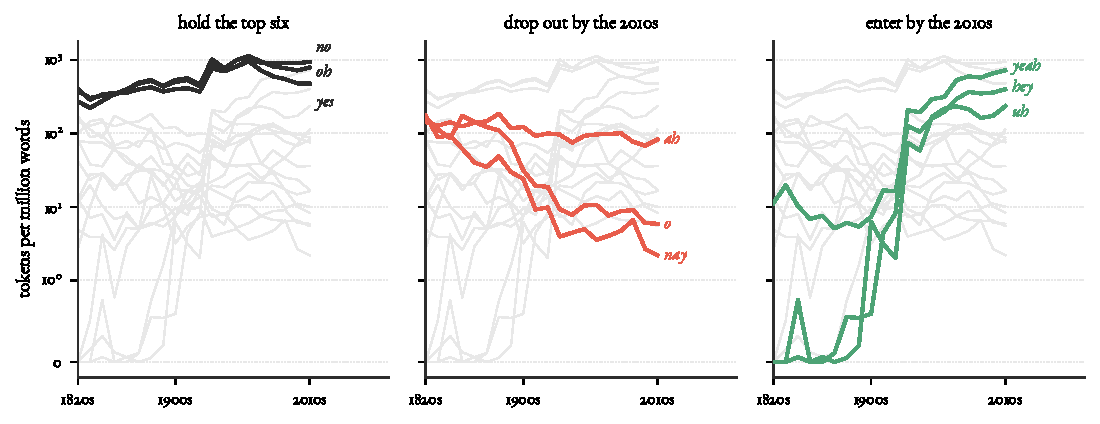
\includegraphics[width=\textwidth]{interjection-turnover.pdf}
  \caption{Turnover in the COHA interjection-tag inventory. Each panel shows all twenty of the most frequent \textsc{uh}-tagged lemmas in COHA (grey), with one group picked out. Half the 1820s top six is displaced by the 2010s by forms absent or negligible at the corpus's beginning. Tokens per million words on a symmetric log scale retain zero values. The tagged inventory isn't an independent test of profile stability. Extracted 2026-07-27 and archived under \texttt{analysis/hand-extracted/}.}
  \label{fig:turnover}
\end{figure}

Regional variation supplies a synchronic comparison among recorded inventories. GloWbE \citep[1.9~billion words across 20 English-speaking countries]{daviesfuchs2015} contains strong raw-string concentrations: \mention{lah} in Singapore and Malaysia, \mention{yaar} in India and Pakistan, and \mention{haba} in Nigeria. Subject to the measurement limits in Section~\ref{sec:discussion}, those counts support a geographic description. They don't identify sociolinguistic conditioning, category boundaries, or maintenance mechanisms.

Onomatopoeic coinage supplies another possible source of conventional forms. Here \term{onomatopoeia} names a relation between a form and a sound, not an exclusive lexical category alongside noun and verb. Forms standing in that relation span grammatical categories: \mention{bang} is a noun in \mention{a loud bang}, a verb in \mention{he banged the door}, and, in the grammatical analysis adopted here, an interjection in \mention{Bang! You're dead}. Imitation can therefore supply forms with an interjectional profile without a preceding nominal or verbal use.

The stock of imitable sounds isn't fixed by the stock of animals: devices supply \mention{beep}, \mention{ping}, and \mention{whirr}, while sounds can be re-rendered, as comics illustrate with \mention{bam} and \mention{pow}. On one analysis, interjections are relatively open because they \enquote{can be rather freely created by onomatopoeia}, as in comic-strip \mention{yucck} and \mention{gr-r-r-r} \citep[74]{quirk1985}. The proposal concerns a productive recruitment route, not the assumption that every imitation acquires the same meaning or interactional use.

Research on ideophones draws a different boundary. \textcite[3, 19]{dingemanse2018} treats onomatopoeia as the sound-imitating subset of ideophones, words that \enquote{depict, using the iconic affordances of speech}; \textcite[529]{dingemanseakita2017} distinguishes interjections as \enquote{primarily indexical}. \textcite[150, 167]{meinard2015} instead excludes onomatopoeias from interjections: \enquote{Isolated onomatopoeias focus on an object of conceptualization and fulfill the referential function of language}, whereas interjections serve conative, phatic, or expressive functions.

These contrasts bear differently on the three classifications. Standalone depictive \mention{Bang!} meets the adopted distributional criterion for \intj{syn}; \textit{CGEL} has no ideophone category, and Diffloth describes ideophones as \enquote{conspicuously undeveloped and poorly structured in the languages of Europe} (Diffloth 1972, as cited in \citealp[12]{dingemanse2018}). Its depiction of a sound doesn't establish the expressive contribution required for \intj{sem}. A state-display use such as \mention{oof} is a candidate for that classification, as \mention{ouch} is, subject to the use-conditional diagnostics. Whether either use has a conventional sequential role is a further question, not settled by depictiveness or standalone position.

Interactional recruitment also motivates comparison among source histories. \textcite{oed_bruh} records \mention{bruh} as a noun from 1894, as a title before a man's name, and from 1967 as familiar address, with vocative quotations (\mention{Hey, bruh}, \mention{Be cool, bruh}). The later standalone stance use needn't address anyone, and the entry doesn't record it as an interjection. COCA frequencies rise from 0.01 per million in 1990--94 to 1.09 in 2015--19.\footnote{Tokens occur overwhelmingly in television and film (1.44 per million) and are absent from the spoken section, so the record represents scripted rather than recorded speech. COHA has no occurrences before the 1980s and nine altogether. Figures are raw-string frequencies; see \path{analysis/hand-extracted/}.}

That family history makes recruitment through address a candidate, not a demonstrated sequence. The stance use has the prosodically separate, non-inflecting, non-referential, externally non-integrated profile at issue here, but the aggregate string counts don't distinguish it from the nominal and address uses. They consequently don't establish its rise separately or the persistence of its profile.

\textcite[191]{dingemanse2020} describes signs that equivocate between sound and speech, such as sighs, sniffs, and clicks, as liminal, treating that status as \enquote{an essential part of their form and function}. Such signs \enquote{may develop into full-blown interjections as they become increasingly conventionalised and on-record}, which \textcite[12]{dingemanse2023preprint} identifies as \enquote{one source path for interjections}. Cultural evolutionary processes \enquote{sample the landscape of possible resources} \citep[191]{dingemanse2020}. The present proposal relates that landscape to the distinct histories and possible dependencies developed above, without assuming that every conventionalized form acquires every cluster property.

The historical cases establish some pathways and motivate others. The frequency probes describe changes and differences in recorded inventories. Those findings make a further question precise without answering it: what can a restricted observation license about an unexamined property or environment, and which proposed classification helps that inference?

\section[Projectibility]{Projectibility as a testable hypothesis}\label{sec:projectibility}

The historical cases in Section~\ref{sec:residues} concern relations between source constructions and later profiles. Forward projectibility asks a different question: what can restricted observations of an identified sign-type tell us about a property or environment not yet observed? This section states declarations that could answer it. Their specification is a contribution to test design, not a report that their held-out success has been established.

Three outcomes must be distinguished. A declaration has \term{predictive success} when its target is sufficiently well anticipated in the specified population. A representation has \term{predictive advantage} when it improves on an appropriate alternative under comparable information and evaluation conditions. \term{Causal support} concerns the processes responsible for the dependence. A cue can predict successfully without a category representation improving on it; a representation can improve prediction without identifying a causal direction; a historically established process can explain a case without yielding a practically useful predictor for new ones.

\subsection{Partial-observation inference}\label{sec:proj-partial}

Projectibility becomes circular if it says only that an interjection has the properties used to classify it. A legitimate declaration fixes the source evidence and withholds the target. The target can belong to a category's wider profile, but it can't be among the observations used to assign the particular case. Different declarations can use different restricted parts of a profile, provided those choices are made before the target results are inspected.

The same discipline applies to the bearer. A sign-type's identity is a hypothesis about a conventional use, not a complete feature vector whose every departure defines another object. The source observations must establish the identification rule and any independently supported contrasts between uses. A target construction that violates the predicted distribution counts against the declaration under that rule. Calling it conversion after seeing the result doesn't remove the failure; a revised account of identity needs independent evidence and a new evaluation (Section~\ref{sec:causal-framework}).

\begin{figure}[htbp]
\centering
\small
\begin{tabular}{@{}p{.27\textwidth}p{.31\textwidth}p{.32\textwidth}@{}}
\toprule
Restricted source evidence & Proposed withheld target & Relevant counterevidence \\
\midrule
An identified use of \mention{gee} has independent prosodic packaging in observed frames & Supplement behaviour in a different grammatical frame & Systematic external integration under the independently fixed identity rule \\
\addlinespace
The same use shows an expressive contrast under separately assessed conditions & Immediacy or intensifying repetition in new contexts & Ordinary descriptive displacement or redundant repetition under those conditions \\
\addlinespace
A sign-type is conventionally recognized as a specified action in one sequential environment & Appropriate action recognition or treatment in a withheld environment & Systematic treatment as incomplete, irrelevant, or a different action \\
\bottomrule
\end{tabular}
\caption{Examples of prospective declarations. Each row requires its own source observations, identity rule, target measurement, and comparison. The targets aren't consequences of the labels by definition, and no held-out success is reported here. The grammatical and semantic examples concern \mention{gee}; the interactional row requires an independently specified action subtype.}
\label{fig:projection}
\end{figure}

Consider standalone stance \mention{bruh}. Prosodic separation, morphological bareness, stance meaning, and its occurrence in a response slot are possible observations. They can't all be counted first as admission evidence and then as predictions. One declaration might use source-context distribution to predict a semantic property; another might use independently established stance meaning to predict treatment in a new sequence. A dataset containing all those properties is useful, but a test must preserve which were available at prediction time.

The category label adds no information after the complete vector from which it was deterministically computed. That isn't a sensible general test of category utility. The relevant comparison asks whether a category- or network-structured representation helps generalize from restricted, noisy, or missing evidence to independently measured targets. It may help by pooling information, restricting possible combinations, or organizing interactions. Each possibility requires a comparison against an alternative allowed to use the same source information.

Analyst and participant claims also differ. \term{Category-driven projection} here concerns an analyst's use of a classification. \term{Cue-driven inference} would concern what speakers or hearers anticipate from partial signals. An analytical category needn't occur in their psychology or cause the behaviour being predicted. A successful analyst-facing test wouldn't by itself establish a participant mechanism; that requires psycholinguistic or interactional evidence appropriate to the claim.

\subsection{What each classification projects}\label{sec:proj-fieldrelative}

The classifications organize different families of prospective inference. Table~\ref{tab:declarations} gives one testable form for each. Its source column describes restricted case-level evidence, not an exhaustive definition. A declaration also needs an identification rule and a target-specific loss or assessment criterion; those are part of its design rather than supplied automatically by category membership.

\begin{table}[htbp]
\centering
\scriptsize
\caption{Prospective declarations and their separate evaluation questions}
\label{tab:declarations}
\begin{tabular}{@{}>{\raggedright\arraybackslash}p{.13\textwidth}>{\raggedright\arraybackslash}p{.25\textwidth}>{\raggedright\arraybackslash}p{.26\textwidth}>{\raggedright\arraybackslash}p{.27\textwidth}@{}}
\toprule
Classification & Restricted source evidence & Withheld target & Comparison and failure \\
\midrule
\intjshort{syn} & Independently identified use and grammatical behaviour in source frames, excluding the target frame & External integration or supplement behaviour in the target frame; complement-taking coded separately & Compare component-property and supplement-function accounts. Target failure challenges the declaration; no comparative gain challenges representational advantage. \\
\addlinespace
\intjshort{sem} & Evidence for a use-conditional expressive contribution, excluding immediacy and repetition tests & Immediacy and intensifying rather than redundant repetition \citep[167]{potts2007} & Compare source-cue predictions and other expressive signs. Ordinary displacement or redundancy challenges the specified generalization. \\
\addlinespace
\intjshort{prag} & Conventional action recognition in a source environment, with subtype independently specified & Recognition or treatment in a withheld environment; subtype-specific floor or repair consequences & Compare local sequential cues, form identity, and action subtype. Broad category value requires benefit beyond the relevant narrower information. \\
\bottomrule
\end{tabular}
\end{table}

For \intj{syn}, the central prediction concerns an independently identified use across grammatical environments. External integration and internal complementation must remain distinct targets: a phrase can be a supplement while its head takes a complement. A prediction of no complement therefore needs its own evidence rather than following from supplement status. Many grammatical targets may be predictable from the component properties alone, leaving the broad classification useful for description but without a demonstrated additional predictive advantage.

For \intj{sem}, the question is whether separately assessed expressive meaning supports further expectations about immediacy, perspective, or repetition. Those properties shouldn't all enter the admission judgment for the same declaration. Prenominal \mention{damn} provides an established comparison with standalone expressive uses; other proposed members require their own evidence. Success would support the specified semantic generalization. It wouldn't show that the label \enquote{interjection} explains more than the relevant expressive classification unless that further comparison were made.

For \intj{prag}, broad membership supports a modest expectation of conventional actionability in an appropriate environment. It doesn't specify one next turn for every member. A continuer can return the floor; a repair initiator can make a repair relevant; a closing can invite a reciprocal closing. Those predictions belong initially to the action subtypes. A test of the broader category asks whether pooling across those subtypes helps recognize or generalize the conventional interactional contribution beyond what subtype, local sequence, and form identity already provide.

The \mention{damn} family illustrates why keeping the levels separate matters. Standalone \mention{damn!} is expressive and available as a stance display. Prenominal \mention{damn} preserves an expressive contribution while differing grammatically. Complement-taking \mention{damn these mosquitoes!} raises an independent category question because \textit{CGEL} tentatively treats the head as an exceptional interjection. Its absence from a backchannel dataset would establish neither the absence of an interactional use nor failure of a stance declaration. The intended subtype and the relevant occasions have to be specified.

Cross-category declarations are possible as well. Grammar-facing source evidence might predict a semantic target, or interactional source evidence might predict grammatical packaging. There are six directed relations among three classifications, and they needn't be symmetrical. Each needs a source set excluding its target, a suitable population, and a failure criterion. The familiar overlap of canonical forms motivates asking those questions; it doesn't answer them.

\subsection{The intersection and representational value}

Joint membership in all three classifications is a conjunction, but mathematical derivability doesn't settle whether that conjunction is a useful grouping. The same applies to any category defined from lower-level features. An unrestricted predictor given the complete membership vector can already represent the intersection, so adding its label cannot supply information absent from those inputs. Treating that redundancy as decisive would also disqualify the component categories under the argument rejected above.

The empirical question concerns a specified representation and task. An explicit intersection might help pool sparse observations, constrain a model, or represent an interaction that separate effects miss. Alternatively it might add complexity without useful improvement. A fair comparison holds available evidence and evaluation cases constant, specifies whether interactions are already represented, and assesses both predictive quality and the costs of the representation. Neither an advantage over an artificially additive baseline nor equality with an unrestricted model settles every question of category standing.

I therefore use the intersection descriptively here and leave its further usefulness open. There is no present evidence of additional projective value, but also no independent test establishing its absence. \textcite[557]{krajinovic2025} make a related demand for explanatory surplus in discussing the iamitive: a proposed aspectual category may be warranted where language-internal mechanisms don't explain a marker's new meanings. Here too, surplus has to be assessed against a specified alternative, not inferred from the presence or absence of a familiar name.

\subsection{What would establish the forward claims}

A direct evaluation should hold out entire lexical or constructional families, rather than random tokens from already familiar item--variety combinations. The source observations, identity rules, and target coding must be independent in the relevant respects. The archived derivative analysis illustrates why pre-registration alone doesn't ensure this: an outcome assigned by the coding rule isn't an independently measured success. The \mention{fie} audit likewise shows that a temporal model can't repair an ineligible denominator or undocumented prediction-derived labels.

Predictive success should first be assessed against the target base rate on genuinely relevant occasions. Targets expressed as absences, such as no determiner or no complement, require an opportunity denominator: cases where a competing analysis or controlled elicitation makes the form a live possibility. Otherwise never encountering the relevant environment can masquerade as a successful restriction. A further comparison evaluates a category- or network-structured model against component cues and developed constructional alternatives given comparable information and flexibility.

For interactional targets, independent coding can distinguish recognition of a conventional action from its particular sequential consequences. For semantic repeatability, a separate judgment or production design may be needed. Evaluation should be paired on the same held-out families, assess calibration as well as discrimination, and represent uncertainty over items, uses, and environments. A high base rate can yield accurate but uninformative predictions; a useful improvement in one subtype needn't generalize to the whole classification.

Systematic target failure weakens the declaration. Accurate targets without comparative improvement leave predictive success intact while limiting the claim for that representation. Neither outcome alone identifies a causal mechanism. To test a proposed coupling, the design needs evidence that discriminates direct dependence from a shared cause or a conventional constructional association. The three questions can be investigated together, but their results should be reported separately.

\subsection{Category, function, and the domain of projection}\label{sec:proj-domain}

The category/function distinction sharpens the comparison. Supplements of several categories share external non-integration and characteristic prosodic packaging. Those properties therefore don't by themselves establish the value of \intj{syn}. Its proposed contribution concerns a wider, independently measured distributional profile, including morphological behaviour and restrictions across frames. Non-referentiality or expressive meaning may supply cross-category targets, but their frequent association with canonical examples doesn't make them defining consequences of the grammar-facing classification.

Productivity requires a different grain. Onomatopoeia can supply new standalone signs, as discussed in Section~\ref{sec:turnover}, but a productive recruitment route is a property of an inventory and process, not a withheld property of one sign-type. It shouldn't be counted as another case-level success beside determiner resistance or supplement behaviour. The same distinction separates a category's persistence across turnover from the continued use of an individual item.

The interactional literature motivates concentrating on sequential targets: frequent central forms include continuers, repair initiators, and change-of-state resources \citep[257--259, 263]{dingemanse2024}. It doesn't establish that the broad pragmatic classification is richer or more predictive than its alternatives. Similarly, \textcite[166--167]{potts2007}'s expressive properties motivate semantic targets without making all traditional interjections expressives. The relations being investigated should determine the domain of projection, rather than a prior ranking of grammar, semantics, and interaction.

The classifications can consequently succeed to different degrees for different purposes. \intj{syn} may preserve a useful grammatical contrast without improving a semantic prediction; an interactional subtype may be strongly predictive while its superordinate classification adds little. A category's standing needn't depend on winning every comparison. The stronger claims are local: that this declaration is informative, this representation helps, or this process explains the dependence. Those are the claims for which the framework requires separate warrant.

\section{Discussion}\label{sec:discussion}

\subsection{What the evidence supports}

The claims developed above don't stand or fall together. Differences among grammatical, expressive, and interactional profiles motivate separate classifications. Independently documented histories can explain particular residues. Neither achievement establishes every proposed causal link, and neither substitutes for testing predictions made from incomplete profiles. The existing probes have to be assessed against the particular claims they can bear on.

The strongest historical case is \mention{gee}. Gehweiler's account documents invocative recruitment and taboo-managed phonological change. Complement-taking \mention{damn} supplies a plausible verbal comparison, but its optative sequence remains reconstructive. These cases support the weaker path-dependence claim: convergence on a similar profile needn't erase source-specific structure. A broader claim would require independently established histories to predict residues across cases, including cases without the expected trace. Residues can't establish a pathway and then count as independent confirmation of that same reconstruction.

This historical account isn't distinctive merely because it connects a present property to a source. Grammaticalization, diachronic prototype, and constructional accounts can preserve such relations too. The proposed network's contribution is to make particular dependencies and their consequences explicit, so that alternative explanations can be compared on the same cases. Its adequacy depends on those links, not on the label \term{network}.

The verbal-derivative study doesn't add the independent confirmation originally intended. Its primary-coding script assigns semantic residue to every retained derivative candidate; the uniformly positive outputs therefore follow from implementation rather than a separately observed semantic outcome (Appendix~\ref{app:morphgain}). Those outputs are retained as an audit record, not evidence. The illustrative distinction remains useful: a derived verb may preserve content associated with a source interjection while changing how that content contributes. Describing a disapproving response doesn't itself express the current speaker's disapproval. Content continuity and continued \intj{sem} membership are different claims.

The \mention{fie} attempt has a different problem. Its model input retains OCR substitutions as zero-valued linguistic observations despite their preregistered exclusion, and numerous assignments have unresolved verification provenance (Appendix~\ref{app:fie}). The resulting curves and ordering probability aren't evidence for or against ordered erosion. Even a corrected token analysis would need to distinguish a changing mixture of uses from changing properties conditional on a conventionalized sign-type. Moreover, the predicted pragmatic--semantic--syntactic order was an auxiliary historical hypothesis, not a consequence of recognizing three categories. Neither an invalid test nor a valid failure of that ordering would decide the full framework.

Inventory turnover establishes a different fact: the forms occupying a conventional tagged inventory change over time. It doesn't show that a category profile persists through replacement. That would require comparable diagnostics across periods, rather than continuity of the tag. The recruitment examples and turnover records consequently motivate a stability question; they don't answer it.

GloWbE supplies a narrower distributional probe \citep{daviesfuchs2015}. Candidate forms concentrate in particular country-labelled web sections, and a crossed-intercept model estimates additional overall country variation: country SD 0.44, 95\% CrI 0.28--0.65. Its estimated predictive improvement is positive but imprecise, approximately 18 ELPD units with SE 13. These results don't establish item-type-specific conditioning, category-boundary decomposition, or identity work. Per-million rates also conflate availability, preference, and frequency of relevant occasions. The counts, models, and country-specific measurement audit are reported together in Appendix~\ref{app:conditioning}.\footnote{\ifblind Available at [link removed for blind review].\else The data and code are archived at \url{https://github.com/BrettRey/interjections-hpc/tree/master}.\fi}

The audit is consequential for the interpretation, not merely a general caveat. Tagged \mention{ha} includes country-dependent proportions of \term{hectare}, names, and laughter; raw regional strings include non-English material and homographs. Precision correction doesn't recover missed tokens. Some geographic comparisons survive defensible coding choices, but that robustness concerns measured frequency. It doesn't establish the proposed regional or indexical process that might maintain an item or its profile.

Hub-property asymmetry likewise remains open. As \textcite[151--152]{meinard2015} reports, the \textit{OED} classes \mention{pop} in \mention{the cork went pop} as an adverb; Meinard instead treats \mention{went} as introducing reported speech. On the adverb analysis, integrated syntax accompanies changed packaging. Partial referentiality in \mention{God}, by contrast, permits nominal and interjectional uses. These contested contrasts motivate comparison, but they don't identify prosodic isolation as an upstream cause or establish its greater causal contribution. Definitional consequences of changing a diagnostic mustn't be mistaken for an intervention on an independently identified mechanism.

The evidence therefore supports historical case analyses and a differentiated descriptive architecture, while leaving the proposed stabilizers and forward projections to direct evaluation. A component-property account may predict some targets just as well. A network earns additional explanatory standing where independently supported links explain contrasts or generalize to withheld cases; matching a descriptive list is insufficient, but failure of one added link needn't eliminate the classifications that remain independently useful.

\subsection{Boundary disputes and explanatory scope}\label{sec:boundaries}

Separating the three inquiries clarifies boundary disputes without automatically resolving them. Routine formulae such as \mention{bye}, \mention{hello}, and \mention{sorry} share standalone availability with canonical interjections, while addressee orientation, conventional response slots, and felicity conditions motivate further distinctions \citep[108--110]{ameka1992}. Social convention and politeness may explain some of that organization, but identifying those candidate grounds is separate from demonstrating their effects.

Fillers such as \mention{um} and \mention{uh} share syntactic non-integration but differ in emphasis, pause distribution, and citation-introduction behaviour \citep[560, 567--572]{oconnell2005}. Their overlap with interjections raises questions about processing and sequential organization rather than requiring a single position on an undifferentiated scale.

Ameka's separation of routine formulae preserves distinctions in speech-act status and social routines \citep[109--110]{ameka1992}; Wilkins's inclusion preserves pragmatic and semantic commonalities \citep[142]{wilkins1992}. Both arguments concern meaning and interaction, so assigning each author to a different field wouldn't settle their disagreement. The proposed decomposition instead makes the competing contrasts explicit. Which classifications earn a place still depends on the distributions, explanations, and non-circular projections they support.

\section{Conclusion}\label{sec:conclusion}

The traditional label \term{interjection} covers distinctions that a single classification needn't preserve. I have proposed three overlapping classifications: grammar-facing \intj{syn}, semantics-facing \intj{sem}, and interaction-facing \intj{prag}. They organize different questions about common sign-types without assigning general priority to one inquiry. They aren't claimed to exhaust every useful grouping, to have uniformly sharp boundaries, or to make their intersection projectively redundant.

The strongest historical evidence concerns particular recruitment pathways and source-compatible residues. The history of \mention{gee} documents an invocative route and euphemistic deformation. Complement-taking \mention{damn} is compatible with a verbal or optative source, though the sequence remains reconstructive. These cases support historical persistence without uniquely establishing the proposed network. Auditing the archived derivative and \mention{fie} analyses reveals that neither supplies a valid test of its intended target. Their numerical outputs can't establish semantic residue or ordered erosion. GloWbE supplies evidence about country-level frequency variation, and COHA illustrates inventory turnover; neither establishes category-boundary decomposition or profile stability.

The proposed coupling and entrenchment links organize further explanatory questions. Their evidence must be assessed separately from the usefulness of the classifications they connect. No complete synchronic network, category-level stability, or corrective control has been established. A developed constructional account remains both a possible implementation and a substantive alternative explanation.

Forward projectibility likewise remains to be evaluated directly. The declarations distinguish predictive success, the advantage of a particular representation, and causal explanation. Their tests require independently identified bearers, withheld targets, appropriate baselines, and a clear distinction between broad category predictions and subtype-specific consequences. A failure constrains the corresponding declaration; it needn't abolish the other classifications or every historical explanation.

The methodological claim is that inquiry-relative categories can overlap without competing for one universally privileged extension. Their standing depends on what they let an inquiry distinguish and infer. Keeping the bearer, the source evidence, the target, and the explanatory commitment separate makes that standing open to assessment rather than securing it by definition.

\ifblind\else
\section*{Acknowledgements}

I compiled empirical material for the Wikipedia article \enquote{English interjections}, of which I'm the primary author. This paper reanalyses that material through the lens of projectibility.

Supplementary materials (data and analysis code for the corpus tests) are available at \url{https://github.com/BrettRey/interjections-hpc/tree/master}.
\fi

% AI disclosure moved to page 1 via \aidisclosure{} after the keywords,
% per house style from 2026-07-16. The end-of-paper Elsevier-form
% declaration that stood here has been removed to avoid duplication.

\clearpage
\begingroup
\setlength{\emergencystretch}{3em}
\printbibliography
\endgroup

\clearpage
\appendix

\section[Supplementary materials]{Supplementary materials: GloWbE conditioning analysis}
\label{app:conditioning}

\subsection{Data and measurement}

Frequency counts for 18 items were extracted from GloWbE \citep{daviesfuchs2015}: 1.9 billion words across 20 countries. The items are the 10 most frequent interjection-tagged forms (\mention{yes}, \mention{no}, \mention{oh}, \mention{yeah}, \mention{hi}, \mention{hey}, \mention{wow}, \mention{hello}, \mention{ah}, \mention{ha}), three regional forms (\mention{lah}, \mention{yaar}, \mention{haba}), semi-regional \mention{eh}, boundary items \mention{cheers} and \mention{bye}, and fillers \mention{um} and \mention{uh}. Core counts are tag-restricted; regional counts are raw strings because the tagger doesn't recognize the relevant uses. Neither measure identifies the three field-relative categories independently.

Country is assigned to a page rather than a speaker. Assignment uses Google's region function: country domains provide a direct cue, but for \texttt{.com} and \texttt{.org} sites Google \enquote{relies on several heuristics, including 1) the IP address for the web server, 2) who links to that website, and 3) who visits the website} \citep[4]{daviesfuchs2015}. Davies and Fuchs themselves question \enquote{how well Google has correctly identified web sites by country}. The page list was seeded through Google searches for \enquote{hundreds of very high frequency 3-grams (three word strings)} from the Corpus of Contemporary American English (p.~4), anchoring the sampling frame to American frequency data. Country differences may therefore reflect genre mix, internet ecology, and sampling alongside linguistic variation.

Automatic tagging adds another measurement layer. An overall error rate doesn't warrant comparisons if validity varies by country \citep{reynolds2026didcorpus}. Concordance coding estimates precision, the proportion of tagged hits that are genuine, not recall, the proportion of genuine tokens retrieved. Neither \mention{haba} nor \mention{yaar} receives an interjection tag. All 373 Nigerian \mention{haba} hits are tagged as common or proper nouns, with 65\% on a reading including the proper noun. The raw-string regional counts can therefore overstate frequency while a tag-restricted query misses these forms entirely.

\subsection{Geographic distributions}

Regional concentration is clear in the raw strings: \mention{lah} occurs at 9.35 per million words in Malaysia and 6.72 in Singapore, and \mention{yaar} at 2.88 in Pakistan and 2.33 in India, with near-zero rates elsewhere. Nigeria's 373 \mention{haba} hits give an upper bound of about 9 per million. Inspecting hits, counting five spellings, and excluding Nigerian Pidgin, indigenous-language material, and duplicates, \textcite[69]{unuabonahdaniel2020} report 248 tokens, or 5.8 per million. The gap illustrates why raw strings and tagged counts aren't directly comparable.

Among the core items, \mention{ah} has the largest cross-country coefficient of variation (CV; standard deviation divided by mean), 0.71: Singapore's 60.42 and Jamaica's 53.16 per million are about eight times Kenya's 7.62. For \mention{yeah}, CV is 0.55 and the United States--Tanzania comparison is approximately 6:1 (103.78 versus 16.85). \mention{Yes} and \mention{no} have lower CVs, 0.21--0.22. The fillers \mention{um} and \mention{uh} have CVs of 0.61 and 0.76, and \mention{bye} has 0.61.

Bootstrap intervals resample the twenty observed country sections. They describe sensitivity to that resampling, not sampling uncertainty over all English-speaking communities: the sections aren't a random sample of such communities. The \mention{yes}/\mention{no} intervals lie below those of eleven of the thirteen other nonregional items, overlapping only \mention{hello} and \mention{ha}. This supports their comparatively low observed dispersion. The remaining marginal intervals overlap; that doesn't establish equal dispersion or settle pairwise differences. A ranking would require paired contrasts within resamples. Regional concentration is better represented by the counts: when a form is absent from eighteen sections, resampling can sharply alter the mean and CV. For \mention{lah}, the interval runs from 0.89 to 4.27.

\begin{figure}[ht]
  \centering
  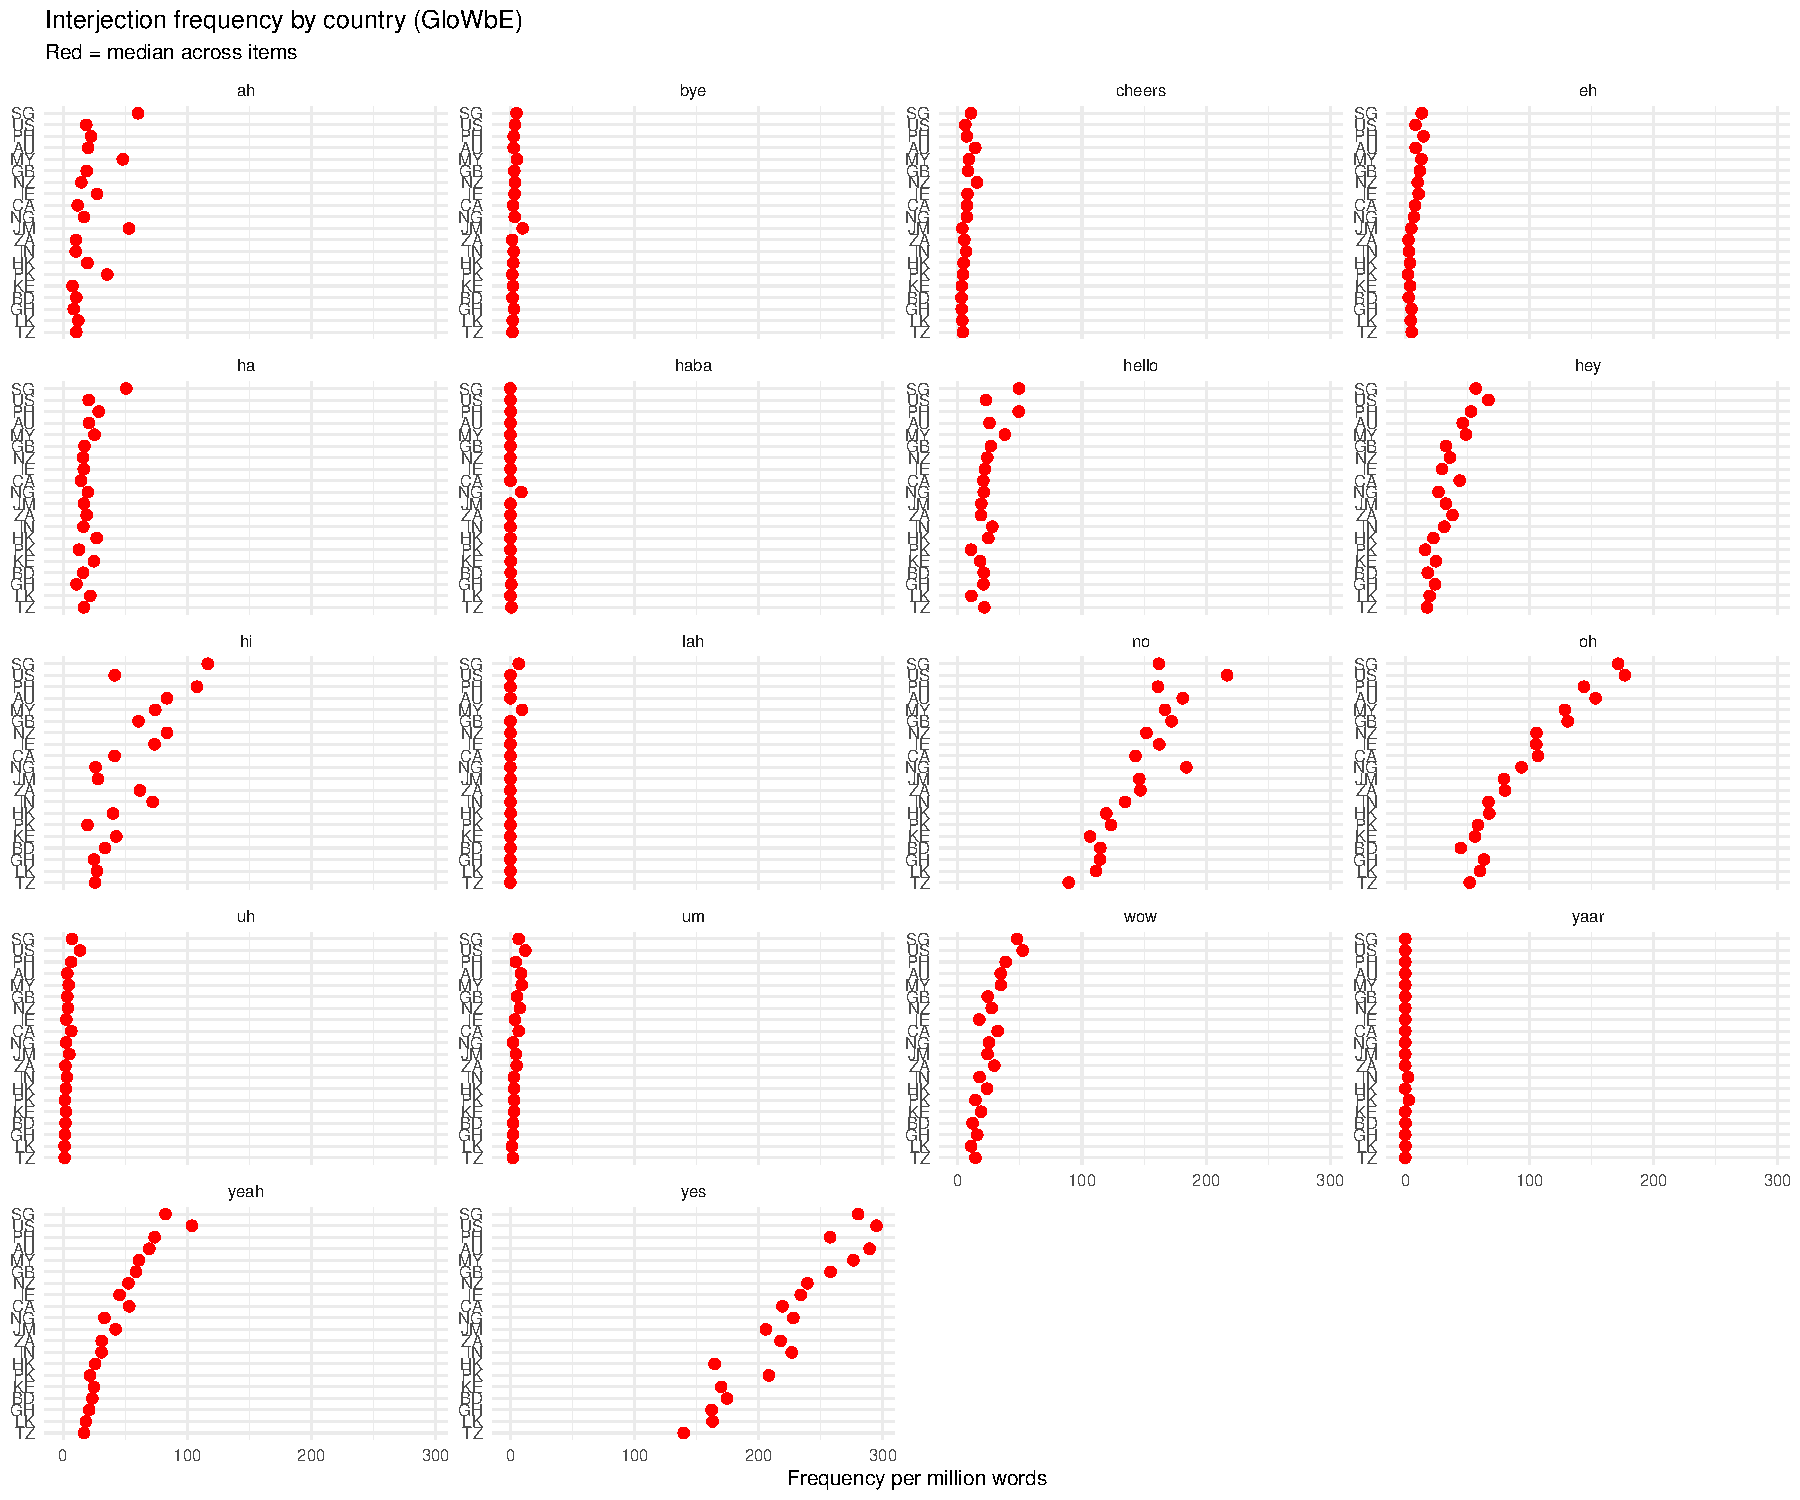
\includegraphics[width=\textwidth]{country-variation.pdf}
  \caption{Frequency per million words across 20 GloWbE country sections. Red points show the median across items within each section. Regional strings (\mention{lah}, \mention{yaar}, \mention{haba}) concentrate in one or two countries; \mention{yes} and \mention{no} have comparatively low dispersion. Tagging and raw-string validity differ by item and country, as the audit below documents.}
  \label{fig:country-variation}
\end{figure}

\subsection{Concordance audit and sensitivity}

The tagger's training on inner-circle English limits its treatment of regional forms, but recognized items aren't necessarily clean. An initial twenty-token check of tagged \mention{ha} in Kenya and Tanzania retained six and eight interjections respectively; most other hits abbreviated \term{hectare} in agricultural and development prose. Applying the Kenyan estimate reduces 24.9 tokens per million to about 7.5 and moves Kenya from fifth to nineteenth among the twenty sections. This preliminary estimate differs from the fuller audit below.

The \mention{ha} audit also requires an explicit decision about laughter. Iterated \mention{HA! HA!} may represent laughter, closer to eye dialect than a lexical item, whereas sarcastic or sceptical \mention{ha} is an interjectional use. Written data make the distinction harder, and digital \mention{haha} may itself be conventionalized. This decision doesn't exclude imitative forms in principle; imitation is one proposed recruitment route. The reported counts include iterated laughter.

Coding tagged concordances across all twenty sections shows the sensitivity. Laughter constitutes 51.5\% of tagged \mention{ha} in the United States and 63.0\% in Great Britain. Across six defensible treatments of laughter and residual tokens, its CV ranges from 0.40 to 0.83 \citep[cf.][]{gelman2014statcrisis}; the reported 0.41 includes laughter. The dispersion measure therefore depends on the criterion. A separate ranking result survives: country-specific validity correction moves Kenya from fifth to fifteenth under every coding.

The proportion of tagged \mention{ha} judged interjectional ranges from 34.5\% in Bangladesh to 84.0\% in Great Britain. \term{Hectare} dominates contamination in East Africa and South Asia; personal names matter in Singapore, where only 6.1\% of hits are \term{hectare}. Pooling country rates to reflect unequal precision~-- about 8,100 tagged tokens for the United States versus 420 for Ghana~-- moves no section by more than 0.6 percentage points. Between-section variation exceeds the sampling variation within sections. These checks correct false positives; they don't estimate missed interjections.

Spelling variants introduce another country-dependent error. Raw \mention{ya} and \mention{yeh} look like variants of \mention{yeah}, but they concentrate where substrate words are homographs: \mention{ya} peaks in Tanzania (19.5 per million) and Malaysia (13.9), and \mention{yeh} in Singapore (5.6), Pakistan (4.9), and India (4.9). No \mention{yeh} token carries the interjection tag. Pooling both strings with \mention{yeah} reduces its CV from 0.55 to 0.46 while importing non-English tokens unevenly, so the analysis keeps them separate.

Adding \mention{umm}, \mention{ummm}, and \mention{ummmm} to \mention{um} changes its CV from 0.61 to 0.60 with Pakistan excluded, but to 0.72 with Pakistan included. Pakistan returns nearly eight times as many \mention{umm} as \mention{um} tokens, against a median ratio of about a third elsewhere. In a twenty-token Pakistani sample, nineteen are the Arabic teknonym \mention{Umm}, as in \mention{Umm Salama}, from hadith or biographical material; the twentieth mentions the filler. Raw-string lengthening thus measures substrate homography as well as orthographic variation.

Regional forms face the same problem. Hand-coding sixty-nine \mention{yaar} hits puts the English-matrix rate at roughly 60\% in Pakistan and 65\% in India; other hits include Tamil \mention{yaar} \enquote{who}, names, and Roman-script Hindi or Urdu. The relevant twenty-token samples are too coarse for correction, but establish that raw rates are upper bounds. Raw \mention{yes}, \mention{no}, \mention{ha}, \mention{ah}, \mention{oh}, \mention{well}, \mention{right}, and \mention{like} likewise include clausal, quoted, discourse-marker, literary, or noisy uses. The audit establishes a measurement result: validity varies across countries, so pooled frequencies can conceal measurement differences alongside linguistic differences.

\subsection{Model specification}

Four Bayesian negative binomial models were fitted in \texttt{brms}~2.23 in R, with four chains of 2,000 iterations, including 1,000 warmup iterations. Models m0--m2 use exact reloo for leave-one-out cross-validation; exploratory m3 is assessed through Pareto-smoothed importance sampling (PSIS) diagnostics only.

\begin{quote}
\small \noindent\texttt{m0} (unconditional):\\ \texttt{count \textasciitilde{} 1 + offset(log(words\_m)) + (1~|~item)}

\noindent\texttt{m1} (conditioned):\\ \texttt{count \textasciitilde{} 1 + offset(log(words\_m)) +}\\ \texttt{(1~|~item) + (1~|~country)}

\noindent\texttt{m2} (item type):\\ \texttt{count \textasciitilde{} 1 + item\_type + offset(log(words\_m)) +}\\ \texttt{(1~|~item) + (1~|~country)}

\noindent\texttt{m3} (exploratory):\\ \texttt{count \textasciitilde{} 1 + item\_type + offset(log(words\_m)) +}\\ \texttt{(1~|~item) + (1~+~item\_type~||~country)}
\end{quote}

The country intercept in m1 estimates an overall frequency shift across items, not an item-specific country effect. Model m3 adds country-varying slopes by item type, but the sparse type cells~-- semi-regional: 1 item; boundary: 2; filler: 2; regional: 3~-- provide little support for those slopes. Neither model estimates grammatical availability separately from preference or frequency of relevant occasions.

\subsection{Results}

Exact leave-one-out comparisons for the confirmatory models are:

\begin{center}
\begin{tabular}{lrr}
  \hline
  Model & ELPD diff & SE diff \\
  \hline
  m1 (conditioned) & 0.0 & 0.0 \\
  m2 (item type) & $-$9.3 & 7.9 \\
  m0 (unconditional) & $-$17.9 & 13.3 \\
  \hline
\end{tabular}
\end{center}

The country-conditioned model has the highest expected log predictive density (ELPD) point estimate, with an imprecise advantage over m0: $\Delta$ELPD = 17.9, SE 13.3 (rounded in the main text to 18 and 13). Adding item type doesn't improve the point estimate. Model m3 isn't formally ranked because nine observations retain Pareto $k > 0.7$ after moment matching, leaving its PSIS estimates unstable.

In m1, the country standard deviation is 0.44 (95\% credible interval [CrI]: 0.28--0.65), against an item standard deviation of 2.07 (1.49--2.96), a ratio of 4.7:1. The country interval describes estimated variation under the model; its positive bounds aren't independent evidence against an absent effect, since standard deviations are constrained to be nonnegative. The predictive comparison and descriptive frequencies supply the relevant evidence. With 18 items $\times$ 20 countries = 360 observations, the ELPD uncertainty remains substantial.

To propagate the \mention{ha} precision estimates, each country's count was thinned by draws from its \textsc{beta} posterior, leaving the other seventeen items unchanged, and m0 and m1 were refitted. Within this sensitivity analysis, country SD changes from 0.42 to 0.44 with iterated laughter included and 0.45 with it excluded; the model-comparison values change from 28.8 to 26.9 and 28.5. These approximate leave-one-out values support only an internal comparison, not replacement of the exact-reloo results above. Precision correction leaves recall unidentified.

The evidence supports geographic concentration of particular strings and additional overall country variation in these measured frequencies. It doesn't establish social indexing, item-type-specific conditioning, category-boundary decomposition, or a process maintaining the interjectional profile. The audit explains why those stronger interpretations require independently validated uses and comparable contexts.

\clearpage

\section[Semantic residue in COHA]{Supplementary materials: audit of the semantic-residue analysis in COHA}
\label{app:morphgain}

\subsection{Design and extraction}

The morphology-gain study was preregistered before confirmatory extraction and coding, after disclosed feasibility queries (\texttt{f1a2193}, 27 May 2026). Its fixed COHA source families were \mention{wow}, \mention{boo}, \mention{ooh}, and \mention{shoo}, over 1820--2019. The target derivatives were \mention{wowed}, \mention{wowing}, \mention{wows}; \mention{booed}, \mention{booing}, \mention{boos}; \mention{oohed}, \mention{oohing}, \mention{oohs}; and \mention{shooed}, \mention{shooing}, \mention{shoos}. Bare forms were excluded. Extraction on 27 May 2026 used key-word-in-context (KWIC) exports; chart requests for \mention{oohed} and \mention{oohing} failed, but their KWIC exports loaded. The extraction summary records minor chart/KWIC count discrepancies.

The go/no-go threshold required 20 analyzable derivatives and two decades with at least three each. The archived pipeline marked all families GO:

\begin{center}
\begin{tabular}{lrrl}
  \toprule
  Family & Included tokens & Decades with 3+ & Status \\
  \midrule
  \mention{boo} & 364 & 10 & GO \\
  \mention{ooh} & 52 & 6 & GO \\
  \mention{shoo} & 410 & 13 & GO \\
  \mention{wow} & 143 & 9 & GO \\
  \bottomrule
\end{tabular}
\end{center}

\subsection{Intended measures and implementation}

The intended confirmatory measures were VP-head syntax and semantic residue: impressed or evaluative response for \mention{wow}, disapproval or contempt for \mention{boo}, appreciative or surprised response for \mention{ooh}, and directive away-sending for \mention{shoo}. Secondary codes concerned interactional residue~-- recognizable response, uptake, display, or direction~-- and a recoverable target, object, addressee, or stimulus.

An implementation audit changes the evidential status of the results. The archived primary-coding script first applies exclusion rules, then assigns both \texttt{verbal\_syntax = 1} and \texttt{semantic\_residue = 1} to every retained row. The exclusion rules were intended to select verbal uses; their accuracy can't be inferred from the syntax code automatically assigned to every retained row. The resulting file contains 1,462 rows: 969 included and 493 excluded. Semantic persistence wasn't independently measured among the included derivatives; it was assigned by the pipeline. Consequently the outputs below don't constitute a confirmatory result.

Even independently established source content would need separating from expressive meaning type. A verb can describe or cause the response expressed by its source interjection without contributing use-conditionally itself. \mention{The performance wowed us} illustrates that distinction. Continuity of source-associated content would support a limited historical relation, not continued \intj{sem} membership.

\subsection{Archived outputs and their limits}

The confirmatory window began with the earliest decade containing at least three included derivatives and extended until it contained ten. Success required both confirmatory codes; the preregistered support rule placed the lower Jeffreys 95\% interval bound above 0.5. The pipeline produced:

\begin{center}
\begin{tabular}{lrlrrl}
  \toprule
  Family & Tokens & Window & $n$ & Assigned successes & Jeffreys 95\% CI \\
  \midrule
  \mention{boo} & 364 & 1920s & 17 & 17 & [0.865, 1.000] \\
  \mention{ooh} & 52 & 1960s--1980s & 10 & 10 & [0.783, 1.000] \\
  \mention{shoo} & 410 & 1890s--1900s & 16 & 16 & [0.857, 1.000] \\
  \mention{wow} & 143 & 1930s--1940s & 11 & 11 & [0.800, 1.000] \\
  \bottomrule
\end{tabular}
\end{center}

All four outputs meet the numerical rule because the semantic outcome was fixed for retained rows. The secondary diachronic model wasn't estimated because the assigned residue variable had no variation. These records preserve the preregistered attempt; they establish neither semantic persistence nor a general tendency for interjections to acquire morphology or syntax.

\subsection{Reliability record and files}

The archived 10\% reliability sample contains 97 retained rows (seed 2026). Both comparison files are constant for inclusion, VP-head status, and semantic residue, so their agreement is 1.000 but Cohen's $\kappa$ is undefined. The reliability script instead returned 1.000 when expected agreement equalled one; that output isn't a valid $\kappa$. The sample also excludes rejected rows, so it doesn't audit false exclusions.

\begin{center}
\begin{tabular}{lrr}
  \toprule
  Code & Agreement & Cohen's $\kappa$ \\
  \midrule
  Inclusion & 1.000 & undefined \\
  VP-head status & 1.000 & undefined \\
  Semantic residue & 1.000 & undefined \\
  Interactional residue & 0.887 & 0.297 \\
  Targeted entity & 0.557 & 0.025 \\
  \bottomrule
\end{tabular}
\end{center}

The audit uses repository revision \texttt{074dfb44cef5b18d292ac176ba5acbfedc76e3b1}. Under \path{analysis/morphgain-confirmatory/}, the retained outputs are \path{morphgain-extraction-summary.csv}, \path{morphgain-go-nogo-summary.csv}, \path{morphgain-coding-summary.csv}, \path{morphgain-confirmatory-results.csv}, \path{morphgain-earliest-windows.csv}, and \path{morphgain-reliability-results.csv}. The corresponding scripts in \path{analysis/} are \path{morphgain-confirmatory-extract.mjs}, \path{morphgain-confirmatory-prepare.py}, \path{morphgain-confirmatory-code-primary.py}, \path{morphgain-confirmatory-analyze.py}, and \path{morphgain-confirmatory-reliability.py}. They document the implementation; they don't repair the absent independent semantic measurement.

\clearpage

\section[Fie in COHA]{Supplementary materials: audit of the \mentionhead{fie} analysis in COHA}
\label{app:fie}

\subsection{Design, coding, and denominator}

The preregistration (\texttt{e18675b}, 15 March 2026) predicted interactional, then semantic, then syntactic loss among attested COHA uses of \mention{fie}, 1820--2019. It excluded metalinguistic mentions, non-English passages, metadata, and optical character recognition (OCR) noise. Represented speech, including fictional dialogue, was eligible. This ordered-erosion hypothesis was an additional historical commitment; it doesn't follow merely from distinguishing three field-relative categories.

The archived analysis contains 616 coded rows. Its exclusion file separately records 141 entries: 134 OCR errors, three metalinguistic mentions, two non-English cases, and two name fragments. However, the model input still includes obvious OCR substitutions coded zero on all three diagnostics, including \enquote{FIe stroked his closed eyelids} (F014), \enquote{FIe drew her to him} (F028), and \enquote{FIe turned his attention} (F043). The model filters only for a non-missing syntactic code. Thus the stated exclusion rule wasn't successfully implemented in the analysed denominator.

The joint syntactic--semantic--interactional codes are 111 for 448 rows, 000 for 139, 011 for 19, 100 for eight, and 010 for two. In addition, 350 rows carry a note beginning \enquote{predicted}; the archive doesn't establish independent manual verification of all these assignments. These are implementation findings, not new linguistic classifications. An OCR substitution isn't an interjection that has lost three properties. The archived declines therefore can't establish either ordered or simultaneous linguistic erosion.

\subsection{Archived agreement and proportions}

The decade column was hidden in the randomized coding sheet. The reported 10\% blind-recode comparison ($n = 62$) yielded:

\begin{center}
\begin{tabular}{lrr}
  \hline
  Diagnostic & Agreement & Cohen's $\kappa$ \\
  \hline
  \intj{syn} & 87.1\% & 0.68 \\
  \intj{sem} & 96.8\% & 0.90 \\
  \intj{prag} & 96.8\% & 0.90 \\
  \hline
\end{tabular}
\end{center}

These archived agreement values don't validate inclusion decisions or resolve the provenance of predicted codes. Figure~\ref{fig:fie-raw} likewise records the unvalidated input: proportions of 85--100\% through the 1890s, a decline between 1900 and 1940, and later fluctuations. Historical fiction and Shakespeare adaptations contribute positive represented uses in the 1980s and 2000s. Publication dates index the sampled texts, not necessarily the contemporary availability of the represented sign-type.

\begin{figure}[htbp]
  \centering
  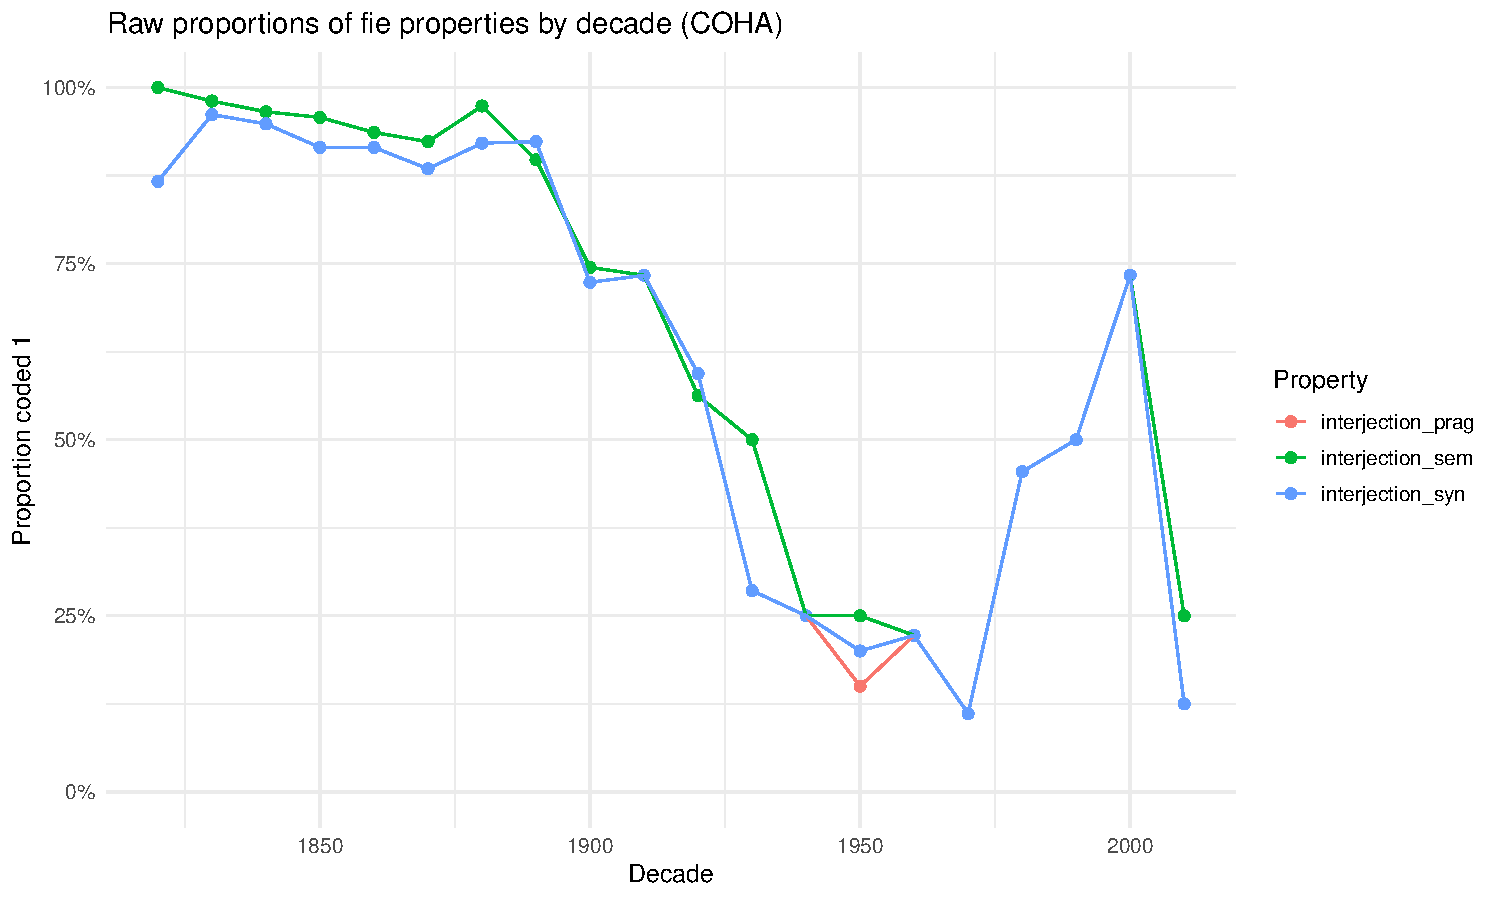
\includegraphics[width=\textwidth]{fie-raw-proportions.pdf}
  \caption{Archived proportions coded~1 by decade in the 616-row \mention{fie} input (COHA, 1820--2019). These are the original diagnostic trajectories, retained to document the attempted analysis. Because OCR substitutions remain in their denominator as zero-valued observations, the curves aren't interpreted as estimates of linguistic property loss.}
  \label{fig:fie-raw}
\end{figure}

\subsection{Archived models and interpretation}

The script fits three separate decade-level binomial logistic regressions, with time centred and scaled in ten-year units. Its normal priors have mean zero and standard deviations 1.5 for the intercept and 0.5 for the slope, with the latter restricted to negative values. Each fit uses four chains, 2,000 warmup and 2,000 subsequent iterations per chain, and seed 2026. The negative-slope restriction imposes monotonic decline and can't model revival. The script centres decade labels rather than the midpoints specified in the preregistration. Separate likelihoods also leave the three outcomes' within-token dependence unmodelled.

\begin{samepage}
The reported ED50 dates ($\tau$, the 0.5 probability crossing) were:

\begin{center}
\begin{tabular}{lrr}
  \hline
  Diagnostic & $\tau$ (median) & 95\% CrI \\
  \hline
  \intj{syn} & 1947 & 1937--1958 \\
  \intj{prag} & 1948 & 1939--1959 \\
  \intj{sem} & 1949 & 1941--1960 \\
  \hline
\end{tabular}
\end{center}
\end{samepage}

The archived probability of $\tau_{\text{int}} < \tau_{\text{sem}} < \tau_{\text{syn}}$ is 0.13, below the preregistration's informal 0.25 threshold for \enquote{inconsistent}. Identical independent priors assign each strict ordering probability $1/6$, so 0.13 wouldn't itself be strong evidence against this order even with a valid denominator. Marginal interval overlap wouldn't establish equality or simultaneity either. More fundamentally, the measurement audit supersedes the substantive interpretation of all these outputs: they supply no present test for or against ordered erosion.

\begin{figure}[ht]
  \centering
  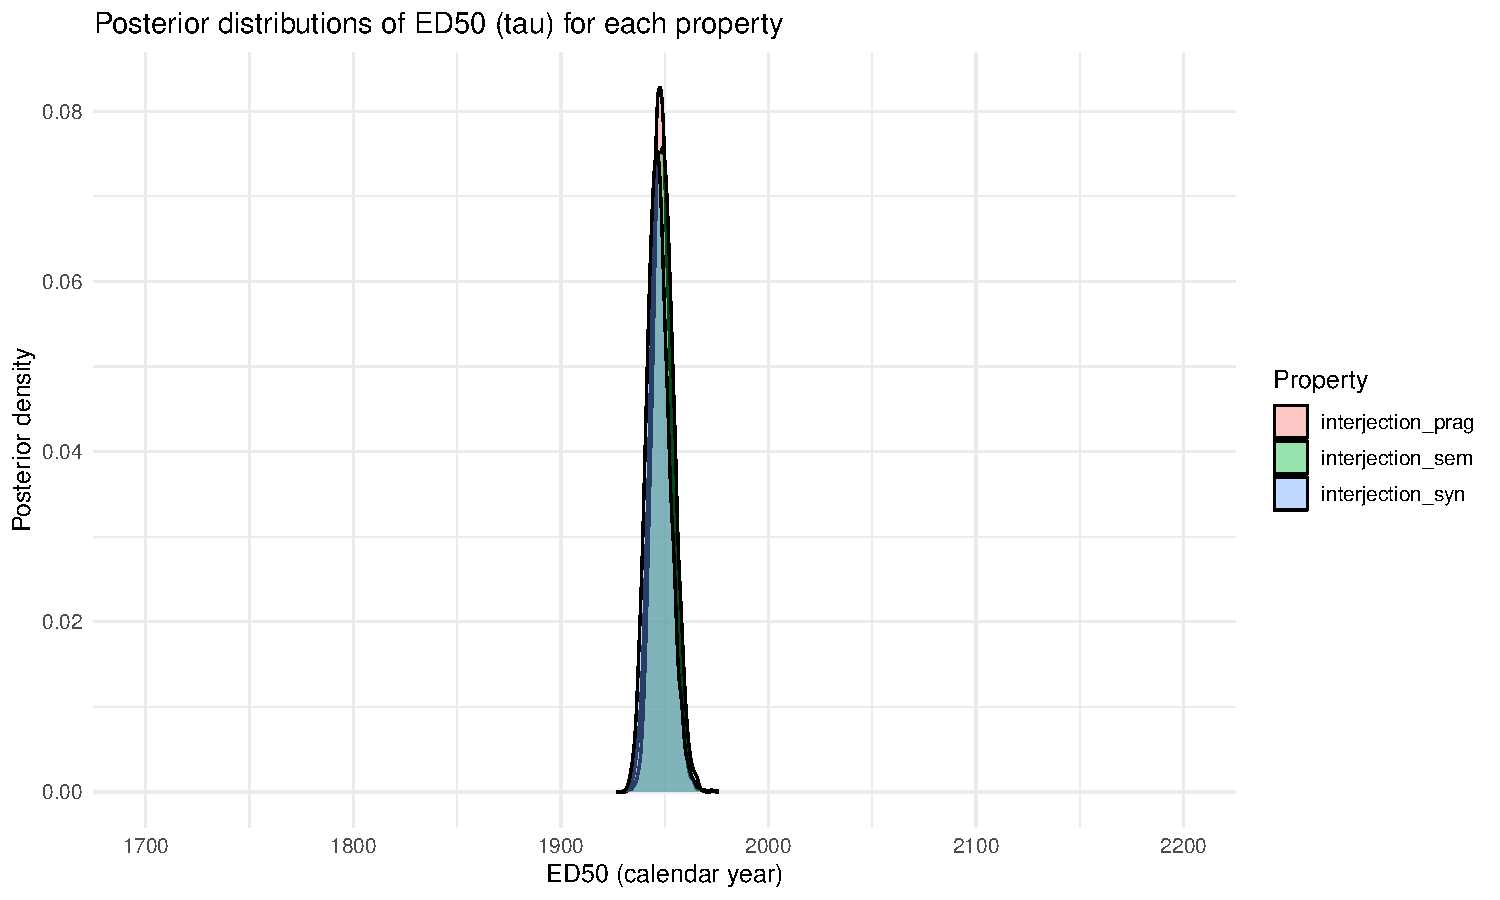
\includegraphics[width=\textwidth]{fie-tau-posteriors.pdf}
  \caption{Archived ED50 distributions from an analysis whose input failed the preregistered exclusion rule. The numerical outputs are retained for the audit record; their overlap isn't evidence for simultaneous loss, and the distributions aren't interpreted as valid estimates of linguistic erosion.}
  \label{fig:fie-tau}
\end{figure}

The audit is tied to repository revision \texttt{074dfb44cef5b18d292ac176ba5acbfedc76e3b1}, especially \path{fie-coha-preregistration.md}, \path{analysis/fie-confirmatory-model.R}, \path{analysis/fie-coding-sheet-annotated.csv}, and \path{analysis/fie-excluded.csv}. A valid comparison would first distinguish eligible occurrences from noise, then separate changing mixtures of sign-types from diagnostic change conditional on a bearer. No recoding or replacement model is reported here.

\end{document}
